\documentclass{article}
\usepackage{graphicx}
\usepackage[hidelinks]{hyperref}
\usepackage{amsmath}
\usepackage[margin=1in]{geometry}
\usepackage{subcaption}
\usepackage{booktabs}
\usepackage{longtable}
\usepackage{float}
\providecommand{\FloatBarrier}{\par}

\setlength{\parindent}{15pt}
\setlength{\textfloatsep}{8pt}
\setlength{\floatsep}{6pt}
\setlength{\intextsep}{6pt}

\title{AERO 510 Final Project Report\\3D Truss and 2D Galerkin FEM Analysis of a Delivery UAV Structure}
\author{Maximilian Mah}
\date{April 2026}

\begin{document}
\renewcommand{\baselinestretch}{1.0}\selectfont
\pagenumbering{gobble}
\maketitle
\thispagestyle{empty}
\begin{center}
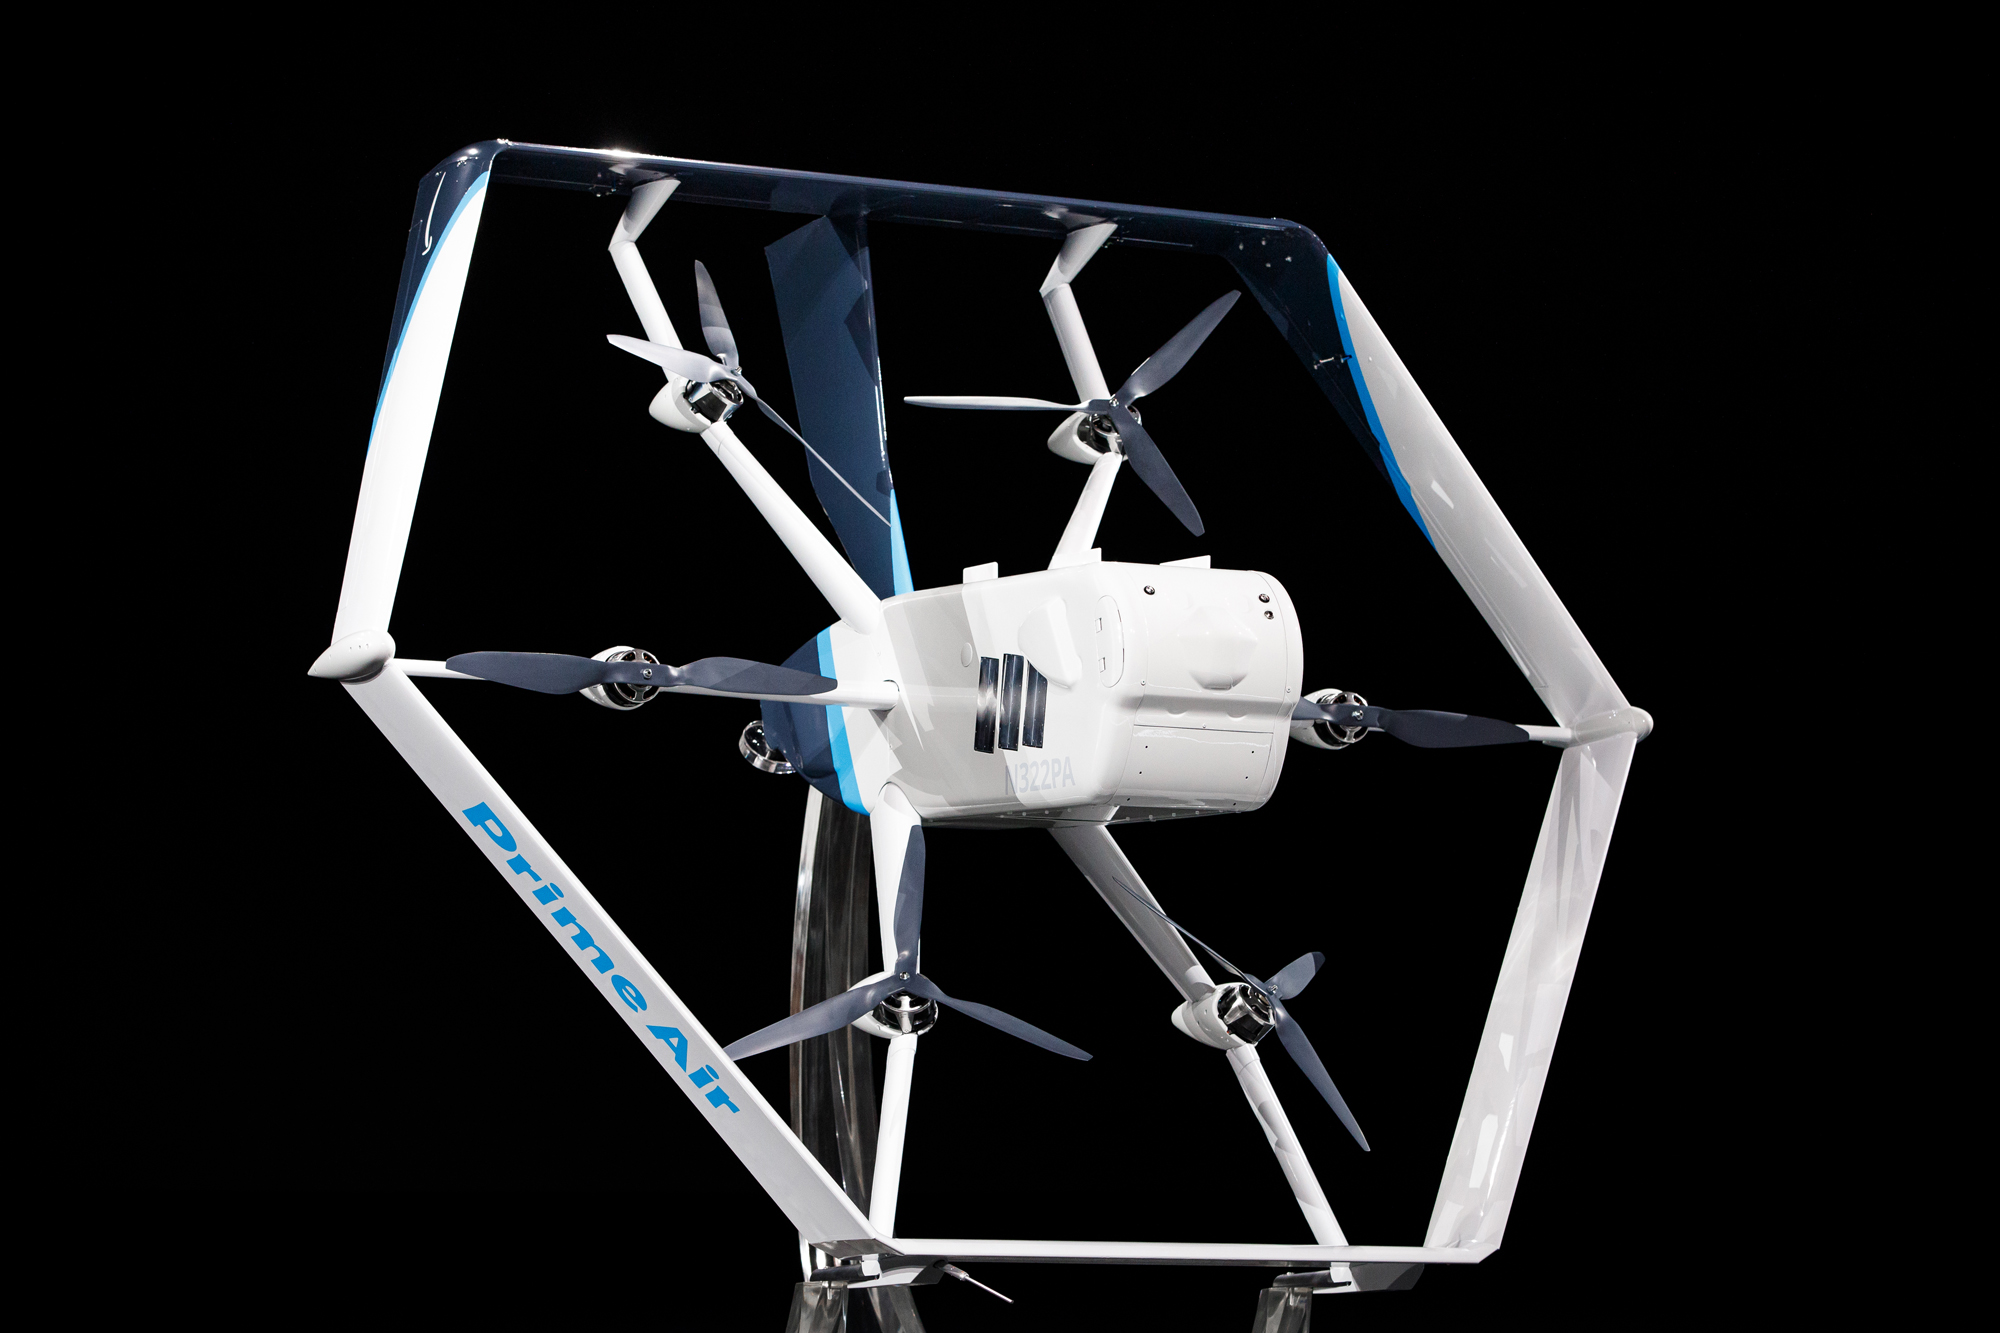
\includegraphics[width=0.56\textwidth]{../figures/amazon-prime-air-remars-june-2019-1.jpg}\\[4pt]
\small Amazon MK27-2 Delivery Drone \cite{techmonitor_mk27_2019}
\end{center}
\clearpage
\pagenumbering{arabic}
\setlength{\columnsep}{3ex}
\twocolumn

\section*{Background and Model Setup}
This project implemented two structural analysis frameworks for a UAV inspired by Amazon's MK27-2 drone: (i) the direct stiffness method for a 3D truss and (ii) a Galerkin finite element formulation using 4-node quadrilateral elements for a 2D panel. The motivation is lightweight structural assessment for parcel-delivery aircraft concepts that have received significant public and industrial attention \cite{tarasov_cnbc_2022,daleo_freightwaves_2022,oitzman_robotreport_2022,grossman_popmech_2019,muller_axios_2022}. Principal hex-frame dimensions were set from MK27-2 public references \cite{faa_mk27_2022,bou_graphicnews_2022}. The geometry was recreated in Rhino 8 and reduced to a tractable structural idealization: spoke attachment locations were simplified and the hub parcel volume was omitted. Figure~\ref{fig:modeling_setup} shows the rendered concept and 2D truss-node/element abstraction used for FEM setup.

For the baseline metal design, aluminum properties were used: $E=70$ GPa and $\nu=0.3$. Member widths were set to 4 in (outer hex edges) and 2 in (spokes), with thickness 0.5 in. A structural mass check was performed from total truss-member volume. The resulting structural weight was 69.07 lb, below the 90 lb vehicle target, leaving margin for unmodeled components and payload.

\section*{Problem 1: 3D Truss Direct FEM}
The truss solver was adapted from lecture/sample direct-stiffness workflows and generalized to 3D assembly/solution. A key modeling detail was a 2 in hub offset in the $z$ direction. If all nodes are coplanar ($z=0$), all member direction cosines along $z$ are zero, so the assembled truss has no axial stiffness coupling to $u_z$ DOFs. In that planar limit, out-of-plane loading cannot produce a valid 3D truss response. The nonzero hub offset makes spoke members carry axial components in $z$, enabling true 3D load transfer.

Three load cases were analyzed:
\begin{enumerate}
    \setlength{\itemsep}{1pt}
    \setlength{\parskip}{0pt}
    \setlength{\parsep}{0pt}
    \item \textbf{Case 1 (mid-flight payload at hub):} a $-5$ lbf point load is applied at node 0 in $z$. This represents a downward package/gravity-driven hub load while the outer frame is treated as rigidly supported. To realize that conservative support assumption, nodes 1--6 are fully fixed: $u_x=u_y=u_z=0$.
    \item \textbf{Case 2 (handling/pull event):} a $+225$ lbf pull is applied at node 1 in $x$, while node 4 is held. This approximates a one-sided pull/drag event during handling or snag recovery. Boundary conditions were selected to retain the physical pull direction while eliminating rigid-body modes: node 4 has $u_x=u_y=u_z=0$; node 1 has $u_y=u_z=0$ so the applied force drives primarily axial $x$ response; node 0 has $u_y=0$; nodes 2,3,5,6 have $u_z=0$.
    \item \textbf{Case 3 (snagged vehicle, thrusting to recover):} node 5 is treated as a snag/contact point and fixed in all DOFs ($u_x=u_y=u_z=0$). A $+15$ lbf load in $z$ is applied at nodes 0,1,2,3,4,6 to represent upward thrust contributions from the remaining free arms. To model thrust-dominated motion and avoid unphysical in-plane drift, nodes 0,1,2,3,4,6 are constrained with $u_x=u_y=0$.
\end{enumerate}

These DOF selections were tuned to be kinematically stable while preserving the intended physical mechanism for each case. In particular, Case 2 and Case 3 require targeted partial constraints (rather than full-frame fixing) to remove rigid-body modes without suppressing the dominant deformation direction being studied.

\begin{figure}[!t]
\centering
\begin{subfigure}{\linewidth}
\centering
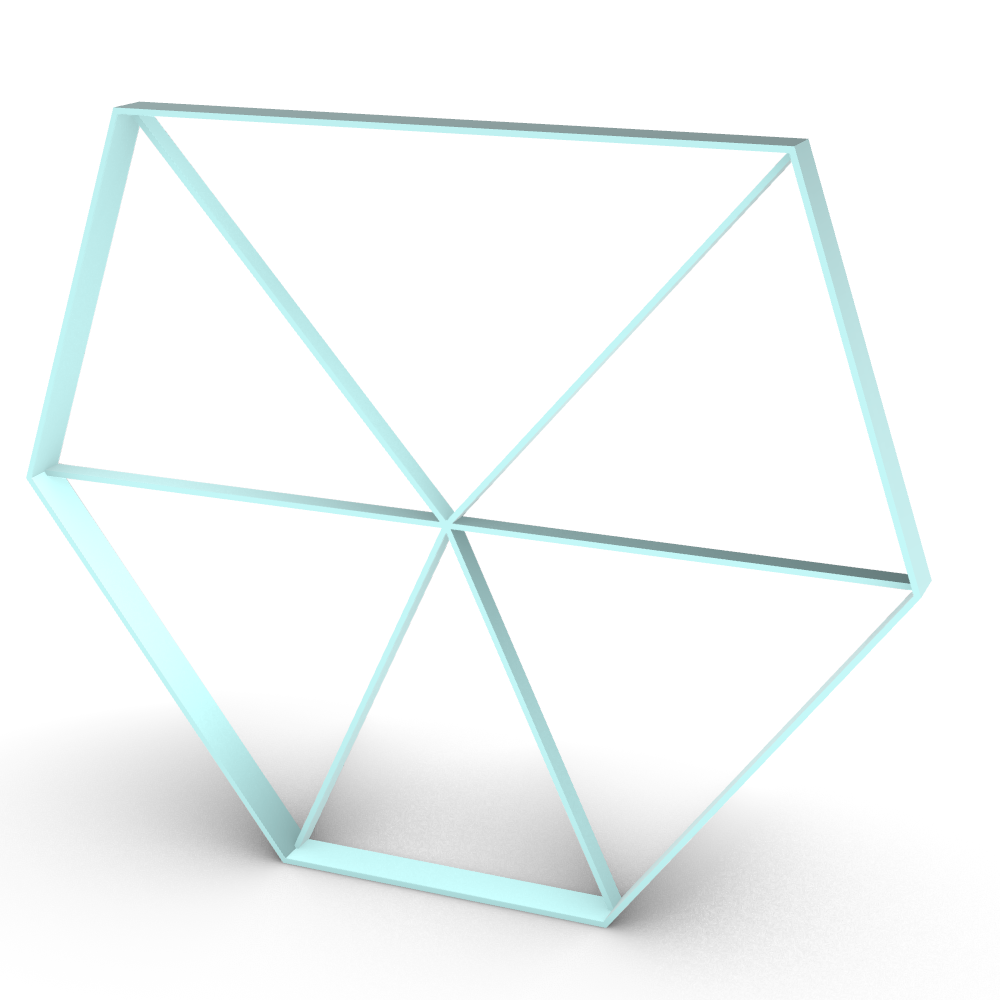
\includegraphics[width=0.74\linewidth]{../figures/truss/hex_render.png}
\caption{Rhino rendering of UAV geometry.}
\label{fig:modeling_rhino}
\end{subfigure}
\vspace{2pt}
\begin{subfigure}{\linewidth}
\centering
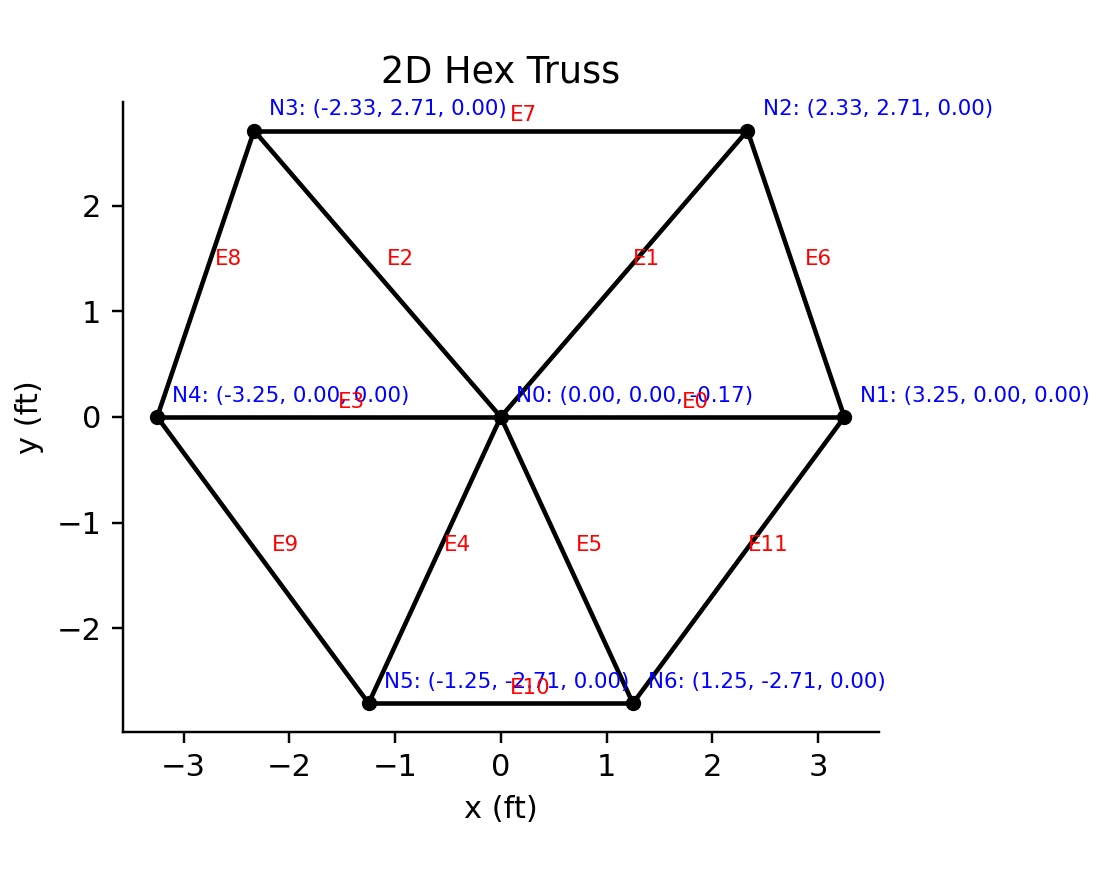
\includegraphics[width=0.74\linewidth]{../figures/truss/hex_2D.png}
\caption{2D truss geometry simplification.}
\label{fig:modeling_hex}
\end{subfigure}
\caption{UAV geometry setup used for truss modeling.}
\label{fig:modeling_setup}
\end{figure}

\begin{table}[!t]
\centering
\caption{Problem 1 displacements and stresses.}
\label{tab:p1_results}
\scriptsize
\setlength{\tabcolsep}{3.0pt}
\renewcommand{\arraystretch}{0.88}
\begin{subtable}[t]{\columnwidth}
\centering
\caption{Problem 1 nodal deflection magnitude, $|u|$ [ft].}
\begin{tabular}{c c c c}
\toprule
Node & Case 1 & Case 2 & Case 3 \\
\midrule
N0 & \textbf{2.199e-06} & \textbf{5.383e-06} & 1.777e-04 \\
N1 & 0.000e+00 & 2.534e-06 & 2.160e-04 \\
N2 & 0.000e+00 & 1.403e-06 & \textbf{2.286e-04} \\
N3 & 0.000e+00 & 1.187e-06 & \textbf{2.286e-04} \\
N4 & 0.000e+00 & 0.000e+00 & 2.160e-04 \\
N5 & 0.000e+00 & 1.197e-06 & 0.000e+00 \\
N6 & 0.000e+00 & 1.450e-06 & 2.073e-04 \\
\bottomrule
\end{tabular}
\label{tab:p1_node_u}
\end{subtable}
\vspace{2pt}
\begin{subtable}[t]{\columnwidth}
\centering
\caption{Problem 1 element axial stress [Pa].}
\begin{tabular}{c c c c}
\toprule
Element & Case 1 & Case 2 & Case 3 \\
\midrule
E0  &  2422.63 & \textbf{21451.89} &  42175.35 \\
E1  & \textbf{2532.94} &  -7292.61 &  46380.31 \\
E2  & \textbf{2532.94} &  -7292.61 &  46380.31 \\
E3  &  2422.63 & \textbf{21451.89} &  42175.35 \\
E4  &  2114.50 & -13605.68 & \textbf{-232310.49} \\
E5  &  2114.50 & -13605.68 &  38718.41 \\
E6  &  0.00 &  2913.25 & 0.00 \\
E7  &  0.00 &  3311.37 & 0.00 \\
E8  &  0.00 &  2913.25 & 0.00 \\
E9  &  0.00 &  7666.37 & 0.00 \\
E10 &  0.00 &  7400.50 & 0.00 \\
E11 &  0.00 &  7666.37 & 0.00 \\
\bottomrule
\end{tabular}
\label{tab:p1_elem_s}
\end{subtable}
\renewcommand{\arraystretch}{1.0}
\end{table}

\begin{figure*}[p]
\centering
\begin{subfigure}[t]{0.49\textwidth}\centering
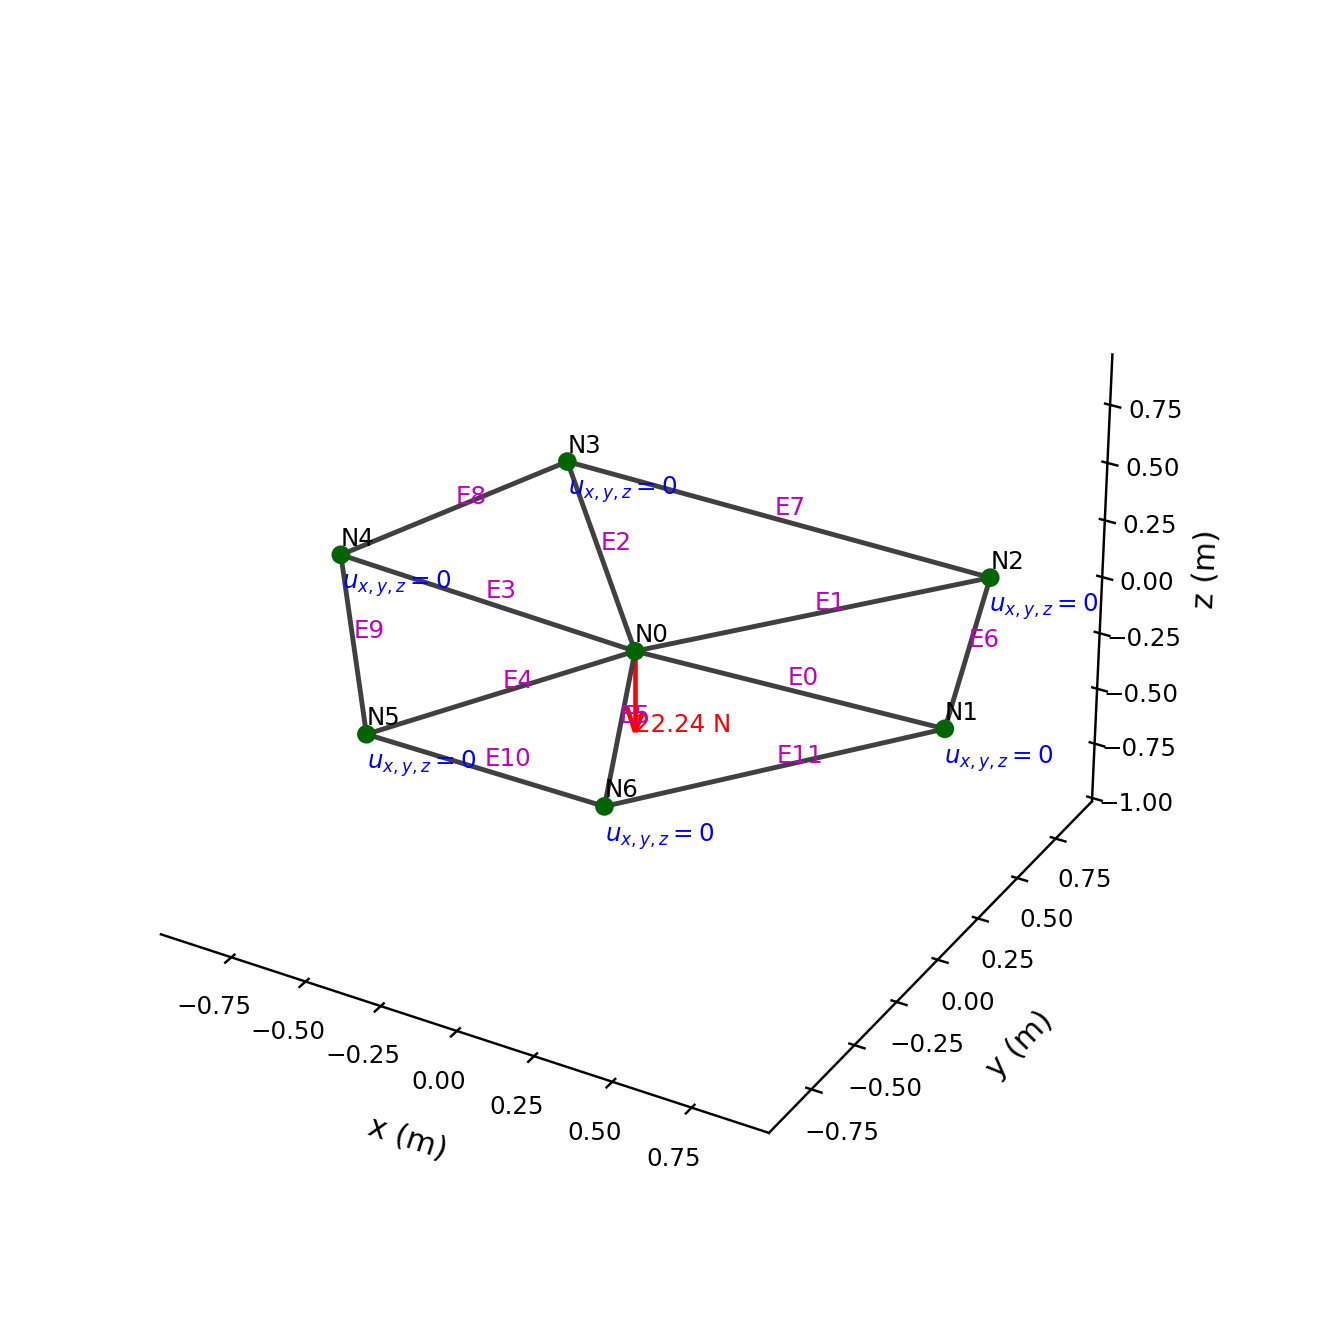
\includegraphics[width=\linewidth,trim=26 24 26 24,clip]{../figures/truss/case1_setup_undeformed.png}
\caption{Case 1 setup}
\end{subfigure}
\hfill
\begin{subfigure}[t]{0.49\textwidth}\centering
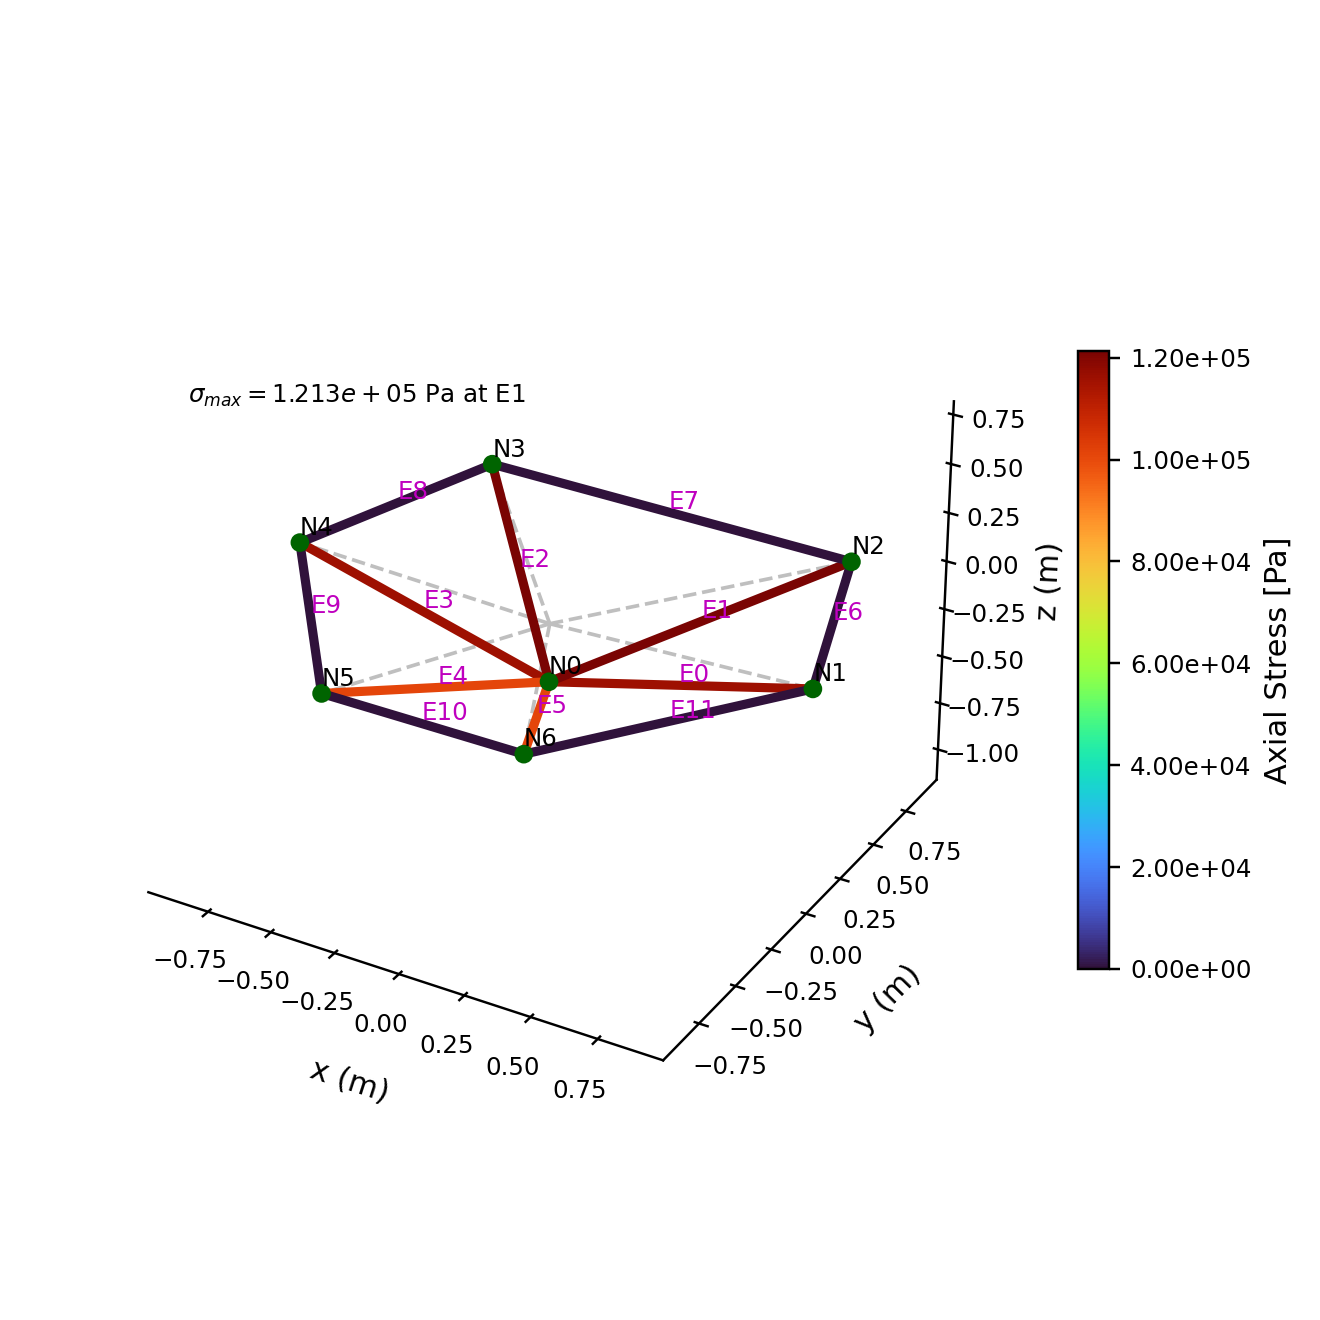
\includegraphics[width=\linewidth,trim=26 24 26 24,clip]{../figures/truss/case1_deform_stress.png}
\caption{Case 1 deformed/stress}
\end{subfigure}

\begin{subfigure}[t]{0.49\textwidth}\centering
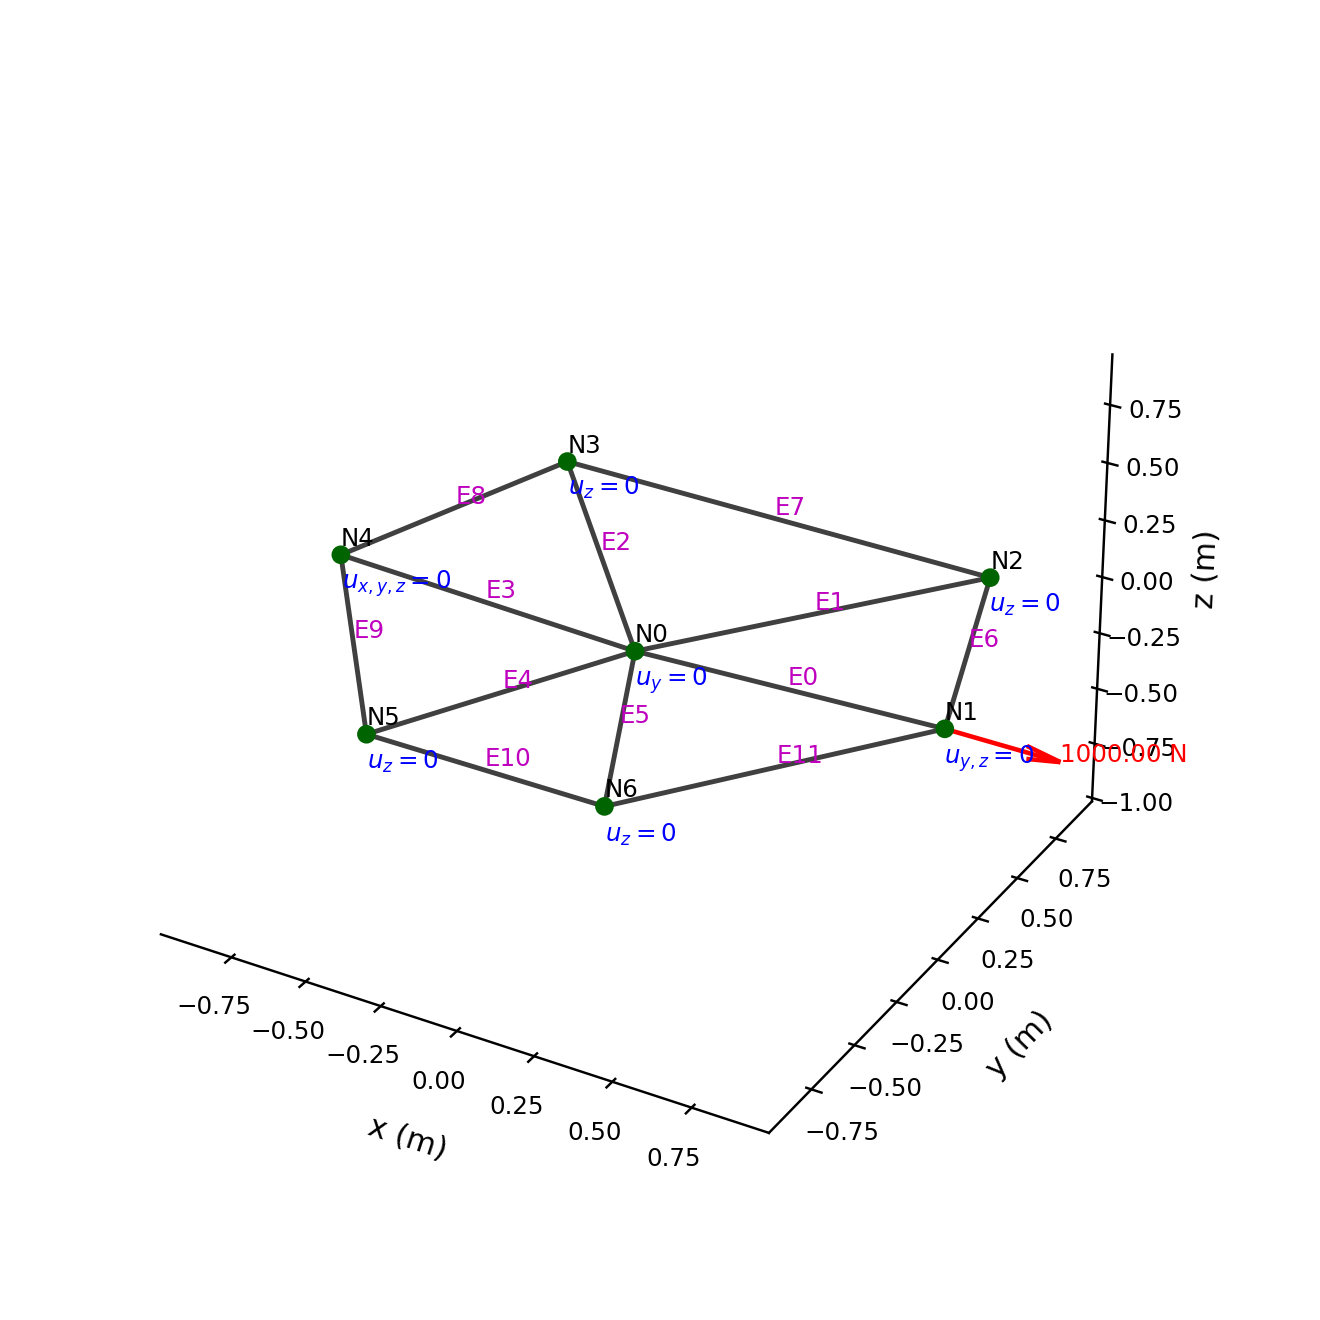
\includegraphics[width=\linewidth,trim=26 24 26 24,clip]{../figures/truss/case2_setup_undeformed.png}
\caption{Case 2 setup}
\end{subfigure}
\hfill
\begin{subfigure}[t]{0.49\textwidth}\centering
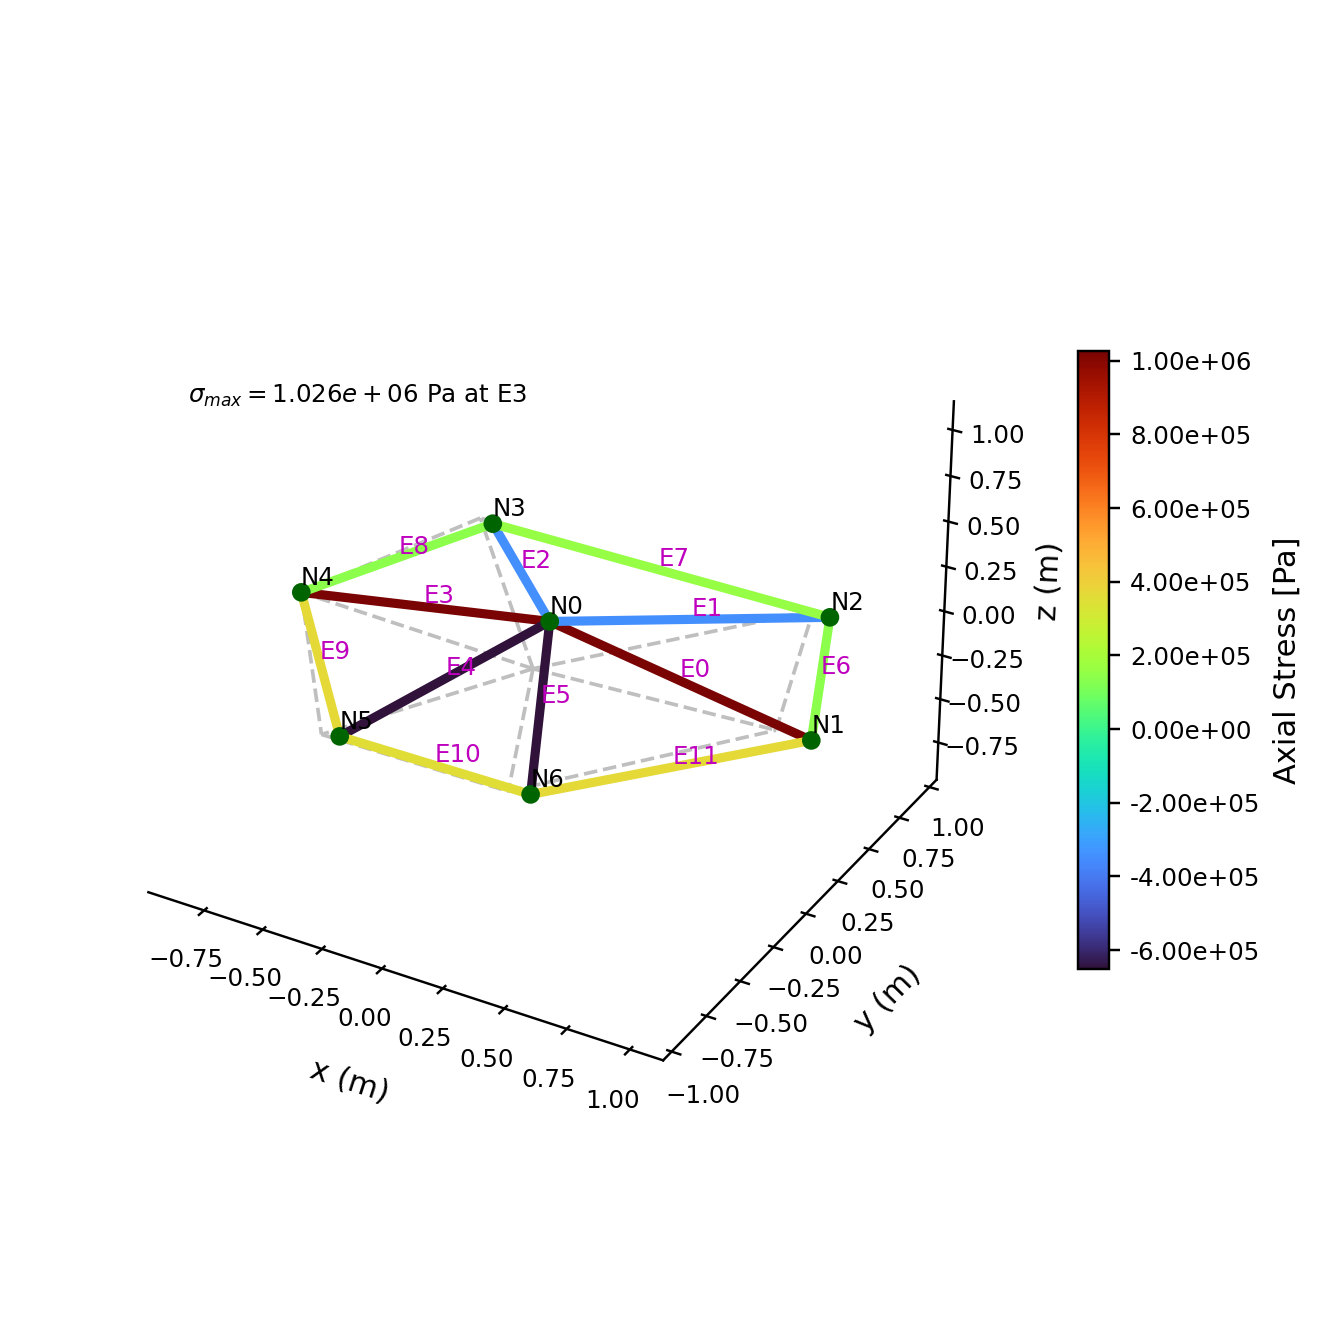
\includegraphics[width=\linewidth,trim=26 24 26 24,clip]{../figures/truss/case2_deform_stress.png}
\caption{Case 2 deformed/stress}
\end{subfigure}

\begin{subfigure}[t]{0.49\textwidth}\centering
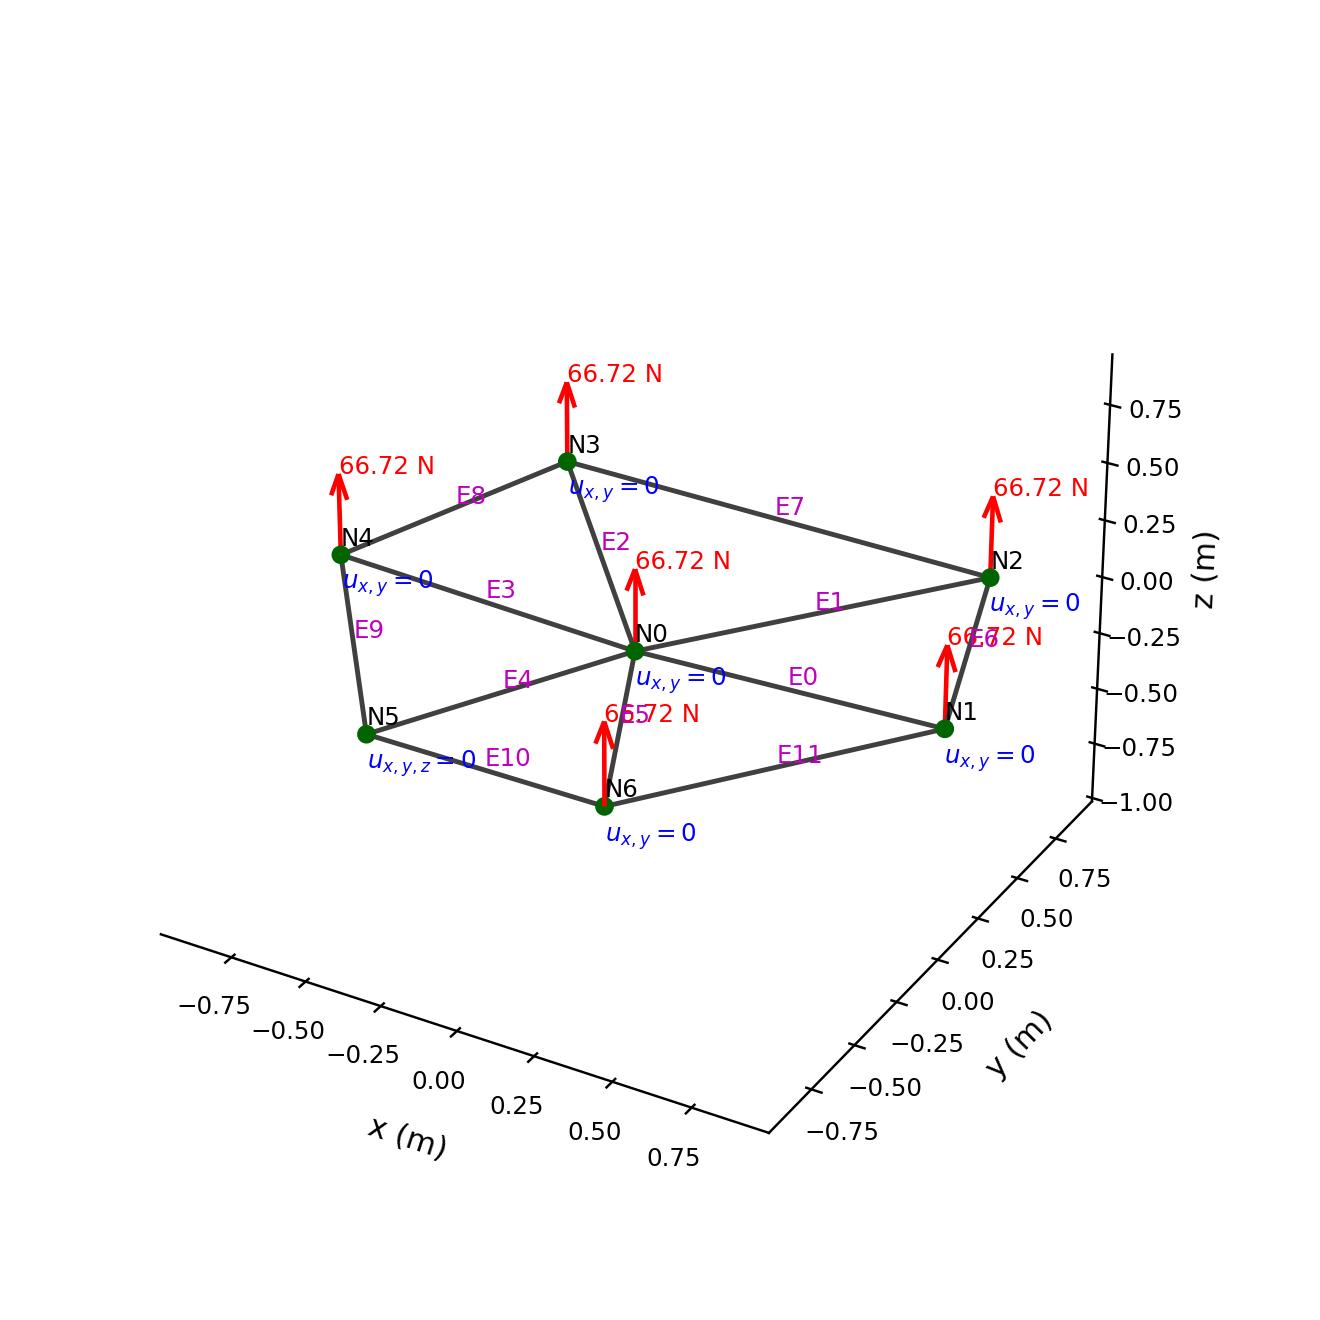
\includegraphics[width=\linewidth,trim=26 24 26 24,clip]{../figures/truss/case3_setup_undeformed.png}
\caption{Case 3 setup}
\end{subfigure}
\hfill
\begin{subfigure}[t]{0.49\textwidth}\centering
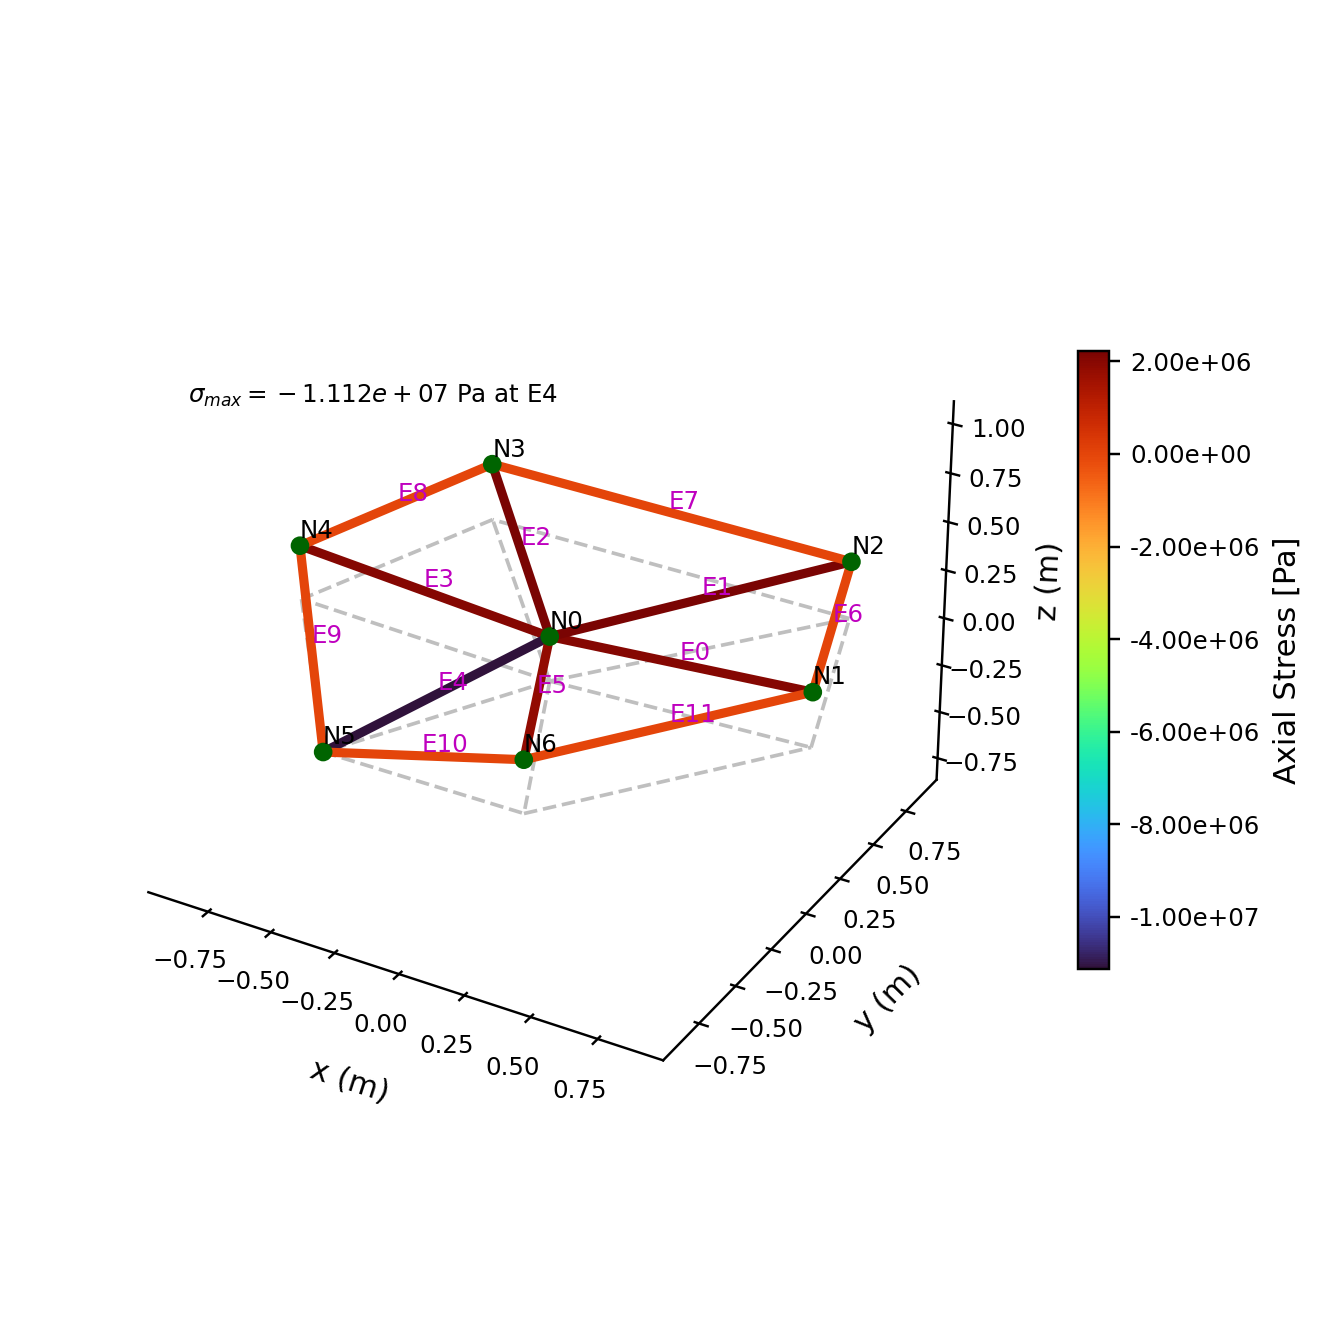
\includegraphics[width=\linewidth,trim=26 24 26 24,clip]{../figures/truss/case3_deform_stress.png}
\caption{Case 3 deformed/stress}
\end{subfigure}
\caption{Problem 1 truss setup and deformed-stress responses for all three loading cases.}
\label{fig:prob1_allcases}
\end{figure*}
\FloatBarrier

\clearpage
\section*{Problem 2: 2D Galerkin Quad FEM (Isotropic Aluminum Panel)}
Using Homework 8 Galerkin-quad structure as baseline, the top panel was modeled as a 2D plane-stress domain. A nominal pressure of 1 MPa was converted to equivalent edge line traction ($q=p\,t$) for 2D application. While high for nominal aerodynamic loads, this was intentionally conservative for stress screening.

Relative to the homework script style, the workflow was reorganized into smaller analysis blocks with single responsibilities. Core routines include \texttt{shape\_quad4} (shape functions/derivatives), \texttt{jacobian\_quad4} (mapping and derivative transform), \texttt{Bmat\_quad4} (strain-displacement matrix), \texttt{gauss2x2} (integration points/weights), \texttt{D\_matrix} (isotropic constitutive matrix), \texttt{assembly} (global stiffness and load construction), \texttt{solve} (free-DOF system solution), and \texttt{postprocess} (element/nodal stresses and von Mises). Boundary/load preprocessing was separated into \texttt{dirichlet\_bcs\_for\_edge} and \texttt{traction\_load}, so each case definition can remain compact and transparent.

Three cases were analyzed:
\begin{enumerate}
    \item \textbf{Case 1 (axial panel pull):} right-edge traction in $+x$, with the left edge fixed ($u_x=u_y=0$). This approximates an in-plane tensile pull of a panel segment attached to a stiffer support on one side.
    \item \textbf{Case 2 (combined tension/shear):} right-edge traction at $45^\circ$, with the left edge fixed. This simulates an off-axis in-plane load where both normal and shear components are important.
    \item \textbf{Case 3 (transverse edge loading):} bottom-edge traction in $-y$, with left and right edges fixed ($u_x=u_y=0$ on both). This represents a panel strip loaded downward between two constrained side boundaries, producing a different stress state than Cases 1--2.
\end{enumerate}

A mesh convergence sweep was performed at $\approx$10, 100, and 1000 elements for each case (9 solves total). Maximum $\sigma_x$, $\sigma_y$, and $\sigma_{vm}$ were tracked versus element count to assess discretization sensitivity before interpreting local stress features. Figure~\ref{fig:p2_convplots} and Table~\ref{tab:p2_conv} summarize the convergence trend for Case 2.

\begin{figure}[H]
\centering
\begin{subfigure}[t]{\linewidth}\centering
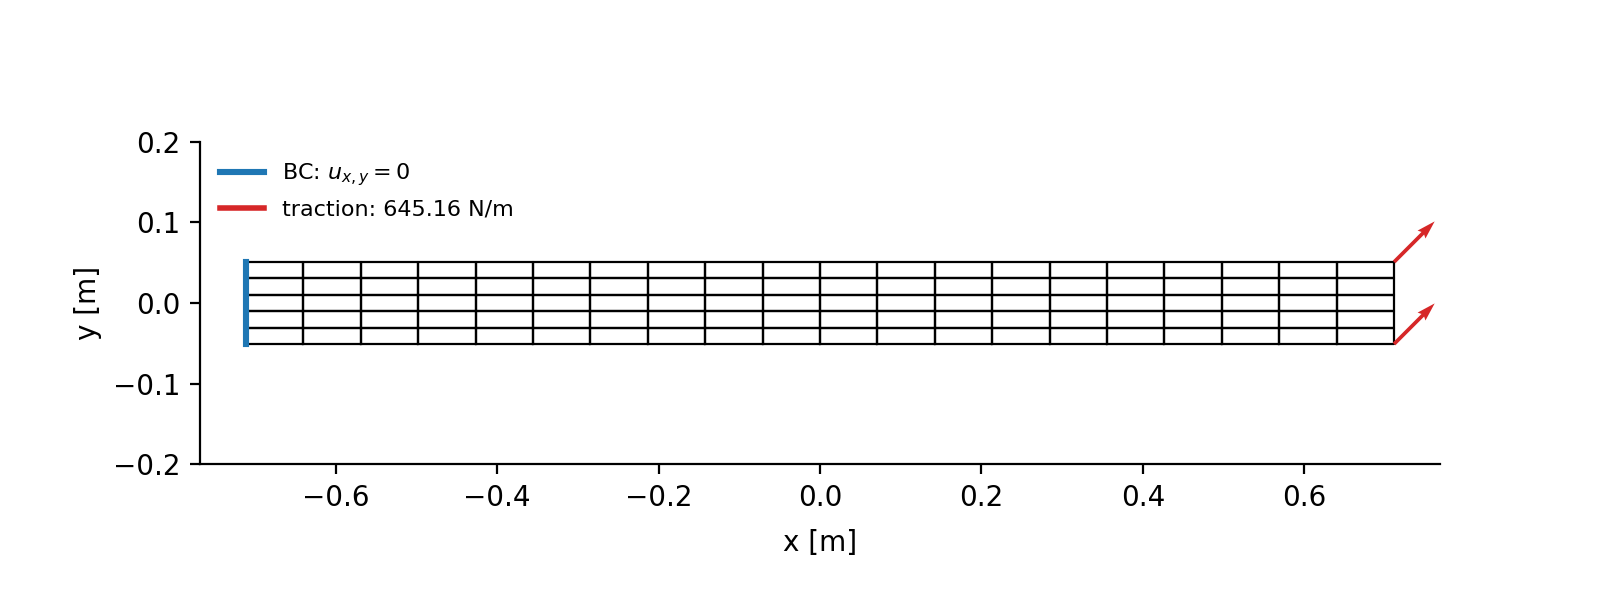
\includegraphics[width=\linewidth,trim=12 24 12 24,clip]{../figures/panel/case2_n100_undeformed.png}
\caption{Undeformed mesh with BCs and traction}
\end{subfigure}

\begin{subfigure}[b]{\linewidth}\centering
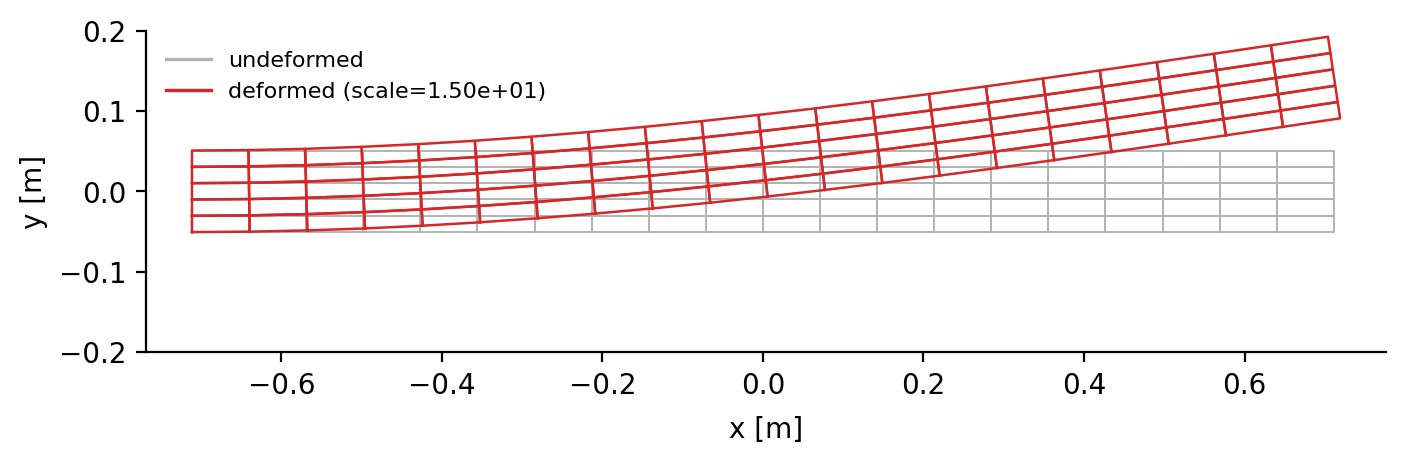
\includegraphics[width=\linewidth]{../figures/panel/case2_n100_deformed.png}
\caption{Deformed mesh}
\end{subfigure}
\caption{Problem 2 case 2 mesh (100 elements)}
\label{fig:p2_sample}
\end{figure}

\begin{figure}[H]
\centering
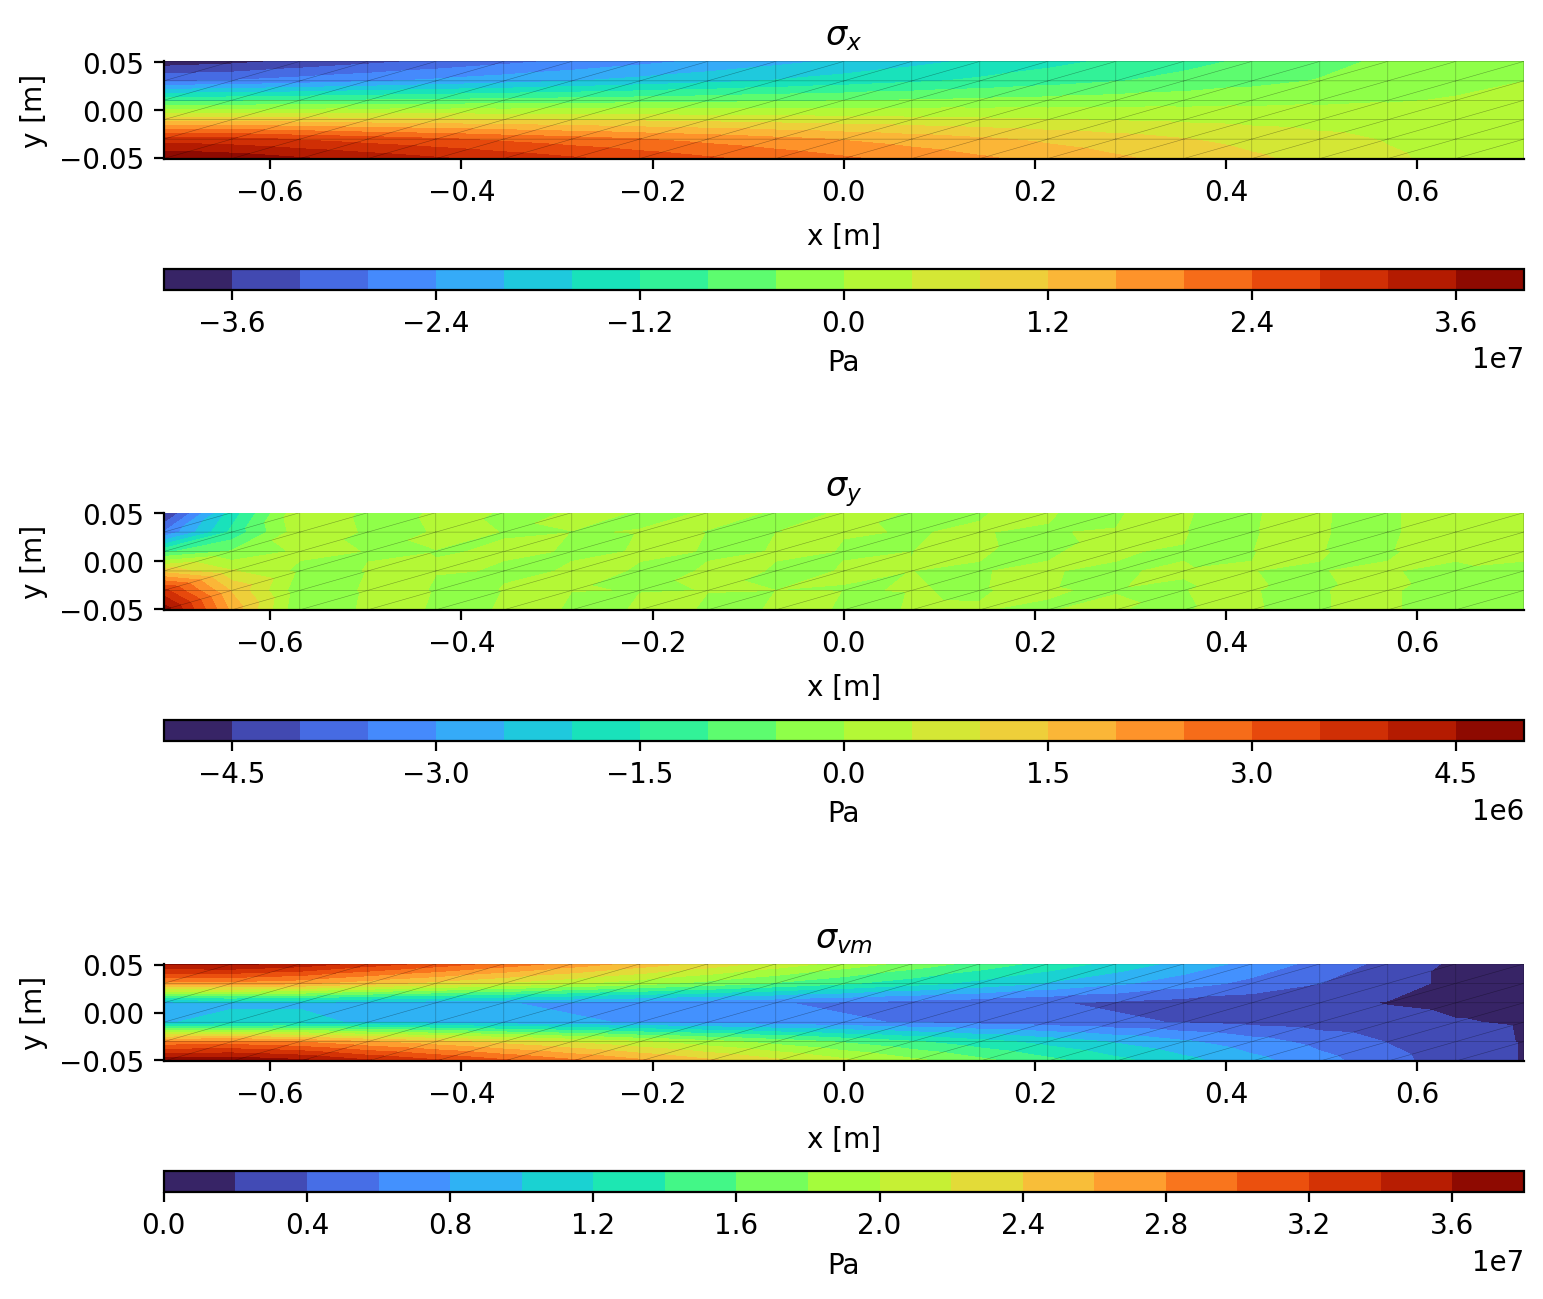
\includegraphics[width=\linewidth]{../figures/panel/case2_n100_stress_stack.png}
\caption{Case 2 stress stack (100 elements).}
\label{fig:p2_stress_stack}
\end{figure}

\begin{figure}[H]
\centering
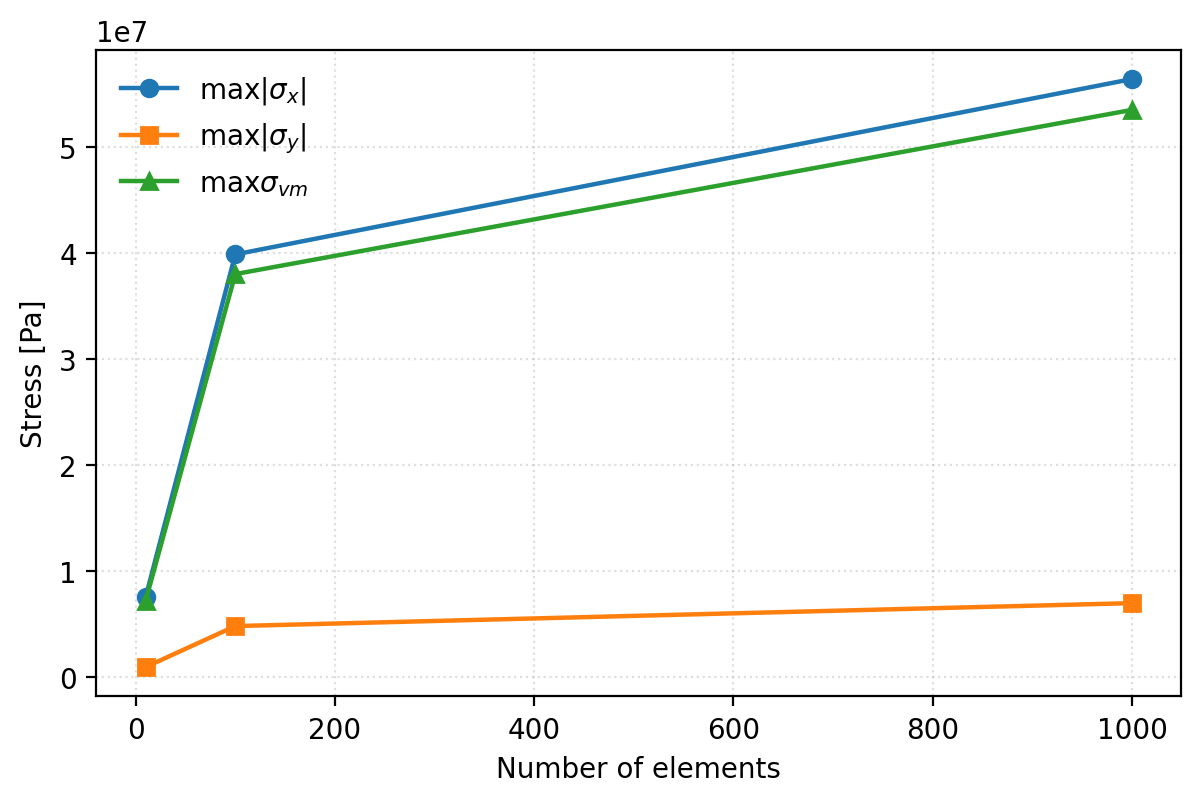
\includegraphics[width=\linewidth]{../figures/panel/case2_convergence_stress.png}
\caption{Case 2 stress convergence}
\label{fig:p2_convplots}
\end{figure}

\begin{table}[H]
\centering
\scriptsize
\caption{Problem 2 convergence study.}
\label{tab:p2_conv}
\begin{tabular}{c c c c}
\toprule
Case & $n_\mathrm{elem}$ & $\max|u|$ [m] & $\max \sigma_{vm}$ [Pa] \\
\midrule
1 & 10   & 2.0209e-05 & 1.01398e+06 \\
1 & 100  & 2.0287e-05 & 1.02219e+06 \\
1 & 1000 & 2.0299e-05 & 1.03680e+06 \\
\midrule
2 & 10   & 2.7944e-03 & 7.21308e+06 \\
2 & 100  & 9.4642e-03 & 3.80192e+07 \\
2 & 1000 & 1.0969e-02 & 5.35066e+07 \\
\midrule
3 & 10   & 4.1768e-04 & 1.12234e+07 \\
3 & 100  & 1.5360e-03 & 5.44499e+07 \\
3 & 1000 & 1.7877e-03 & 8.60951e+07 \\
\bottomrule
\end{tabular}
\end{table}
\FloatBarrier

\clearpage
\section*{Problem 3: CFRP Orthotropic Panel}
\begin{figure}[!t]
\centering
\begin{subfigure}{\linewidth}\centering
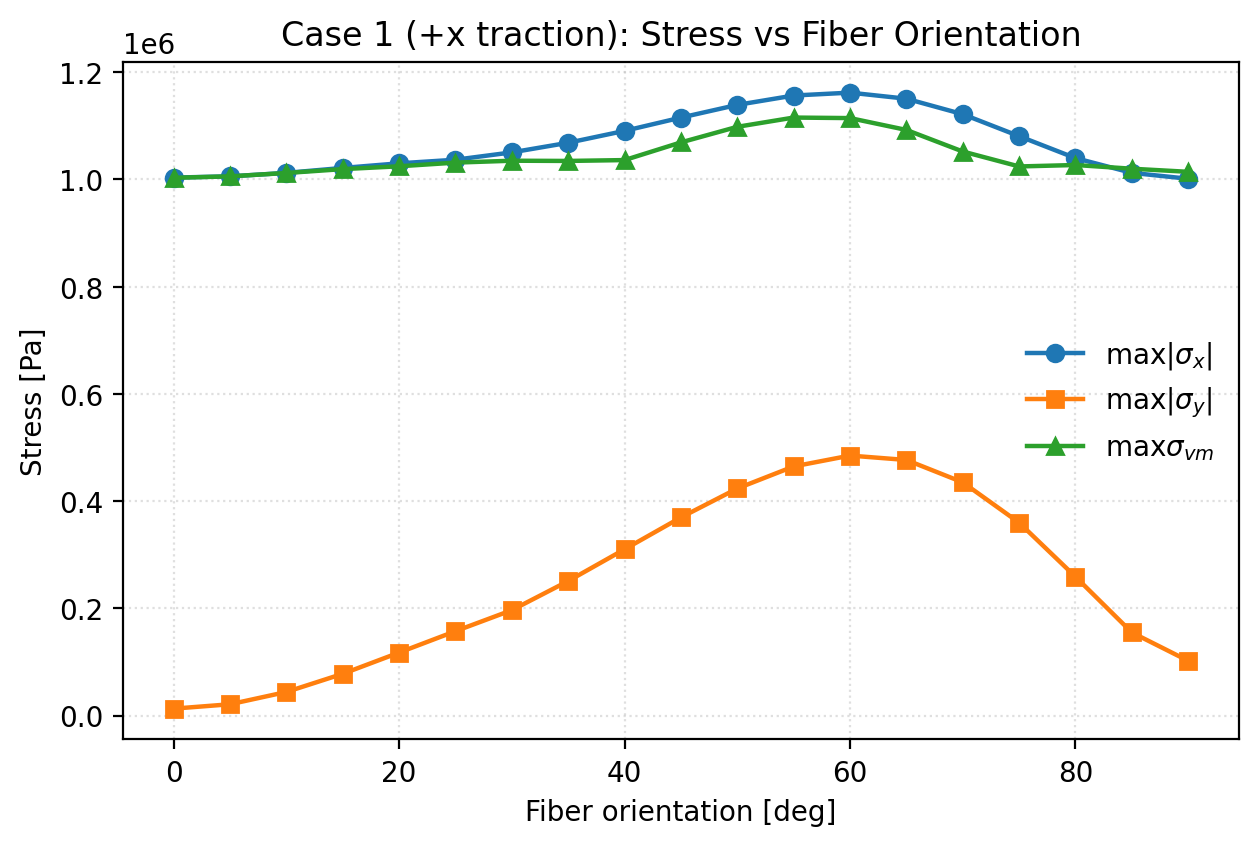
\includegraphics[width=\linewidth]{../figures/panel_composite/case1_orientation_sweep.png}
\caption{Case 1 orientation sweep}
\end{subfigure}
\begin{subfigure}{\linewidth}\centering
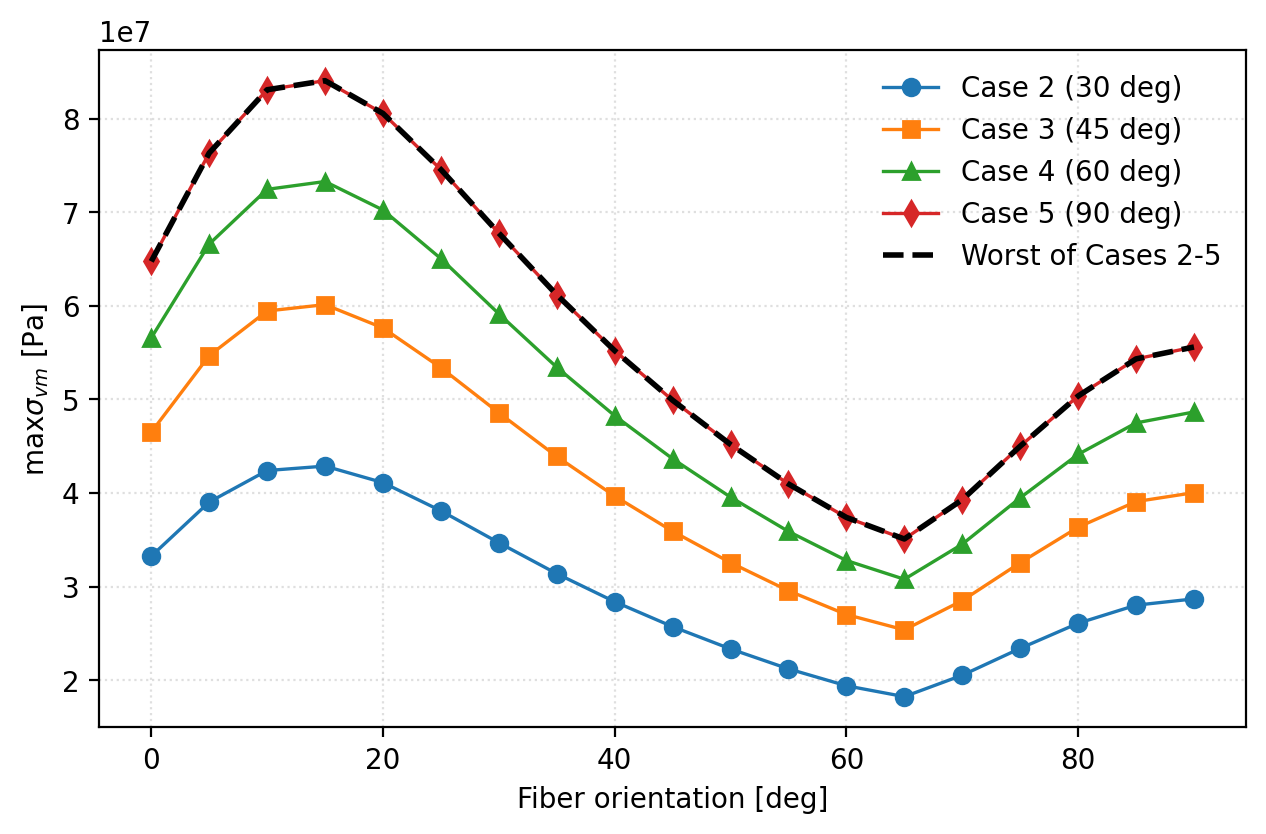
\includegraphics[width=\linewidth]{../figures/panel_composite/cases2to5_orientation_robustness.png}
\caption{Arbitrary traction robustness (Cases 2--5)}
\end{subfigure}
\caption{CFRP fiber-angle trade study.}
\label{fig:p3_orient}
\end{figure}

\begin{table}[!t]
\centering
\scriptsize
\caption{Fiber orientation study}
\begin{tabular}{c c c}
\toprule
$\theta_f$ [deg] & \shortstack[c]{+x traction: \\ $\max \sigma_{vm}$ [Pa]} & \shortstack[c]{Worst traction dir: \\ $\max \sigma_{vm}$ [Pa]} \\
\midrule
0  & \textbf{1.003e+06} & 6.475e+07 \\
15 & 1.019e+06 & 8.407e+07 \\
30 & 1.035e+06 & 6.777e+07 \\
45 & 1.069e+06 & 4.991e+07 \\
60 & 1.114e+06 & 3.738e+07 \\
75 & 1.024e+06 & 4.500e+07 \\
90 & 1.014e+06 & 5.560e+07 \\
\bottomrule
\end{tabular}
\label{tab:p3_orientation}
\end{table}

The panel was then reanalyzed as a unidirectional CFRP lamina under plane stress using orthotropic constitutive response \cite{barbero_composite_fea}. Constituents and volume fraction were set from lecture guidance: carbon fiber/epoxy with $V_f=0.60$, $E_f=241$ GPa, $\nu_f=0.2$, $E_m=3.12$ GPa, $\nu_m=0.38$. From Barbero Chapter 6 micromechanics, effective lamina constants were computed first in the material 1--2 frame, then used to form the reduced in-plane orthotropic stiffness matrix $Q$.

Implementation changes relative to Problem 2 were limited to constitutive modeling and orientation handling; mesh generation, quadrature, assembly, and solver flow were retained. Specifically, orthotropic routines were added to compute $Q$ (`orthotropic\_Q\_plane\_stress`) and rotate it to global axes (`rotate\_Qbar\_plane\_stress`) for a specified fiber angle $\theta_f$. The rotated matrix $\bar{Q}$ replaced the isotropic $D$ in the same element-level stress relation $\sigma=\bar{Q}\,\varepsilon$, allowing direct comparison against the isotropic baseline under identical load/BC definitions.

Five right-edge traction directions were evaluated ($0^\circ,30^\circ,45^\circ,60^\circ,90^\circ$) with left-edge fixed DOFs, and a fiber-angle sweep $\theta_f\in[0^\circ,90^\circ]$ at $5^\circ$ increments was run for each load direction. This provides a direct stress-based proof of orientation selection instead of a single-angle comparison.

\[
\begin{aligned}
E_1 &= 145.848\ \text{GPa} \\
E_2 &= 15.903\ \text{GPa} \\
G_{12} &= 4.339\ \text{GPa} \\
\nu_{12} &= 0.272
\end{aligned}
\]

Table~\ref{tab:p3_orientation} shows representative values and demonstrates the trend used for selection.

Using the full $5^\circ$ sweep, the selected recommendations were:
\begin{itemize}
    \item For pure $+x$ traction (Case 1): $\theta_f=0^\circ$ minimizes $\max \sigma_{vm}$.
    \item For arbitrary right-edge tractions (Cases 2--5): minimax orientation $\theta_f=65^\circ$ minimizes worst-case $\max \sigma_{vm}$.
\end{itemize}

\FloatBarrier
\section*{AI Ethics in Engineering}
For the assignment ethics component, I prompted AI with predefined geometry and case definitions for the 3D truss and 2D panel models. The request was:
\begin{quote}
\small
Solve Problem 1 (3D direct truss FEM for three load/BC cases, plus setup and deformed-stress plots), Problem 2 (2D Galerkin quad FEM for three cases with $n=\{10,100,1000\}$ meshes, output deflections/stresses and convergence plots), and Problem 3 (CFRP orthotropic panel with traction-direction sweep and $5^\circ$ fiber-angle study to recommend orientation).
\end{quote}

AI matched my Problem 1 and Problem 2 results (same trends and similar values), but it initially struggled on Problem 3 relative to my interpretation. The first outputs were overly long, relied on many helper functions/print statements, and needed multiple rounds of correction for setup and output formatting. Initial plotting outputs also required iterative tuning.

After follow-up prompts focused on restructuring and visualization details, the plotting quality improved significantly and supported my original analysis conclusions.

In practice, LLMs should be used as an integrated partner for implementation tasks: coding, refactoring, automation, and postprocessing. They are valuable when the engineer already understands the physics and numerical methods, and then uses AI to accelerate execution. They should not replace engineering intuition, validation, or critical decision-making. The engineer must remain in-the-loop, review assumptions, and avoid black-box use.

\clearpage
\onecolumn
\bibliographystyle{IEEEtran}
\bibliography{references}

\clearpage
\appendix
\section*{Appendix A: Postprocessing Results}

\subsection*{Problem 1: Truss CSV Outputs}

\subsubsection*{Case 1}
\begin{table}[htbp]
\centering
\scriptsize
\caption{Case 1 nodal displacements from \texttt{case1\_node\_displacements.csv}.}
\begin{tabular}{c c c c c}
\toprule
Node & $u_x$ [ft] & $u_y$ [ft] & $u_z$ [ft] & $|u|$ [ft] \\
\midrule
0 & -4.35368518e-24 & -3.57821382e-08 & -2.19911795e-06 & 2.19940904e-06 \\
1 & 0.00000000e+00 & 0.00000000e+00 & 0.00000000e+00 & 0.00000000e+00 \\
2 & 0.00000000e+00 & 0.00000000e+00 & 0.00000000e+00 & 0.00000000e+00 \\
3 & 0.00000000e+00 & 0.00000000e+00 & 0.00000000e+00 & 0.00000000e+00 \\
4 & 0.00000000e+00 & 0.00000000e+00 & 0.00000000e+00 & 0.00000000e+00 \\
5 & 0.00000000e+00 & 0.00000000e+00 & 0.00000000e+00 & 0.00000000e+00 \\
6 & 0.00000000e+00 & 0.00000000e+00 & 0.00000000e+00 & 0.00000000e+00 \\
\bottomrule
\end{tabular}
\end{table}

\begin{table}[htbp]
\centering
\scriptsize
\caption{Case 1 element results from \texttt{case1\_element\_results.csv}.}
\begin{tabular}{c c c c c}
\toprule
Element & Node $i$ & Node $j$ & Strain & Stress [Pa] \\
\midrule
0 & 0 & 1 & 3.46090694e-08 & 2.42263486e+03 \\
1 & 0 & 2 & 3.61848257e-08 & 2.53293780e+03 \\
2 & 0 & 3 & 3.61848257e-08 & 2.53293780e+03 \\
3 & 0 & 4 & 3.46090694e-08 & 2.42263486e+03 \\
4 & 0 & 5 & 3.02071947e-08 & 2.11450363e+03 \\
5 & 0 & 6 & 3.02071947e-08 & 2.11450363e+03 \\
6 & 1 & 2 & 0.00000000e+00 & 0.00000000e+00 \\
7 & 2 & 3 & 0.00000000e+00 & 0.00000000e+00 \\
8 & 3 & 4 & 0.00000000e+00 & 0.00000000e+00 \\
9 & 4 & 5 & 0.00000000e+00 & 0.00000000e+00 \\
10 & 5 & 6 & 0.00000000e+00 & 0.00000000e+00 \\
11 & 6 & 1 & 0.00000000e+00 & 0.00000000e+00 \\
\bottomrule
\end{tabular}
\end{table}

\subsubsection*{Case 2}
\begin{table}[htbp]
\centering
\scriptsize
\caption{Case 2 nodal displacements from \texttt{case2\_node\_displacements.csv}.}
\begin{tabular}{c c c c c}
\toprule
Node & $u_x$ [ft] & $u_y$ [ft] & $u_z$ [ft] & $|u|$ [ft] \\
\midrule
0 & 1.26688509e-06 & 0.00000000e+00 & 5.23155936e-06 & 5.38276984e-06 \\
1 & 2.53377019e-06 & 0.00000000e+00 & 0.00000000e+00 & 2.53377019e-06 \\
2 & 1.37726412e-06 & -2.65805646e-07 & 0.00000000e+00 & 1.40267925e-06 \\
3 & 1.15650607e-06 & -2.65805646e-07 & 0.00000000e+00 & 1.18665872e-06 \\
4 & 0.00000000e+00 & 0.00000000e+00 & 0.00000000e+00 & 0.00000000e+00 \\
5 & 1.13473332e-06 & 3.79589440e-07 & 0.00000000e+00 & 1.19653995e-06 \\
6 & 1.39903687e-06 & 3.79589440e-07 & 0.00000000e+00 & 1.44961798e-06 \\
\bottomrule
\end{tabular}
\end{table}

\begin{table}[htbp]
\centering
\scriptsize
\caption{Case 2 element results from \texttt{case2\_element\_results.csv}.}
\begin{tabular}{c c c c c}
\toprule
Element & Node $i$ & Node $j$ & Strain & Stress [Pa] \\
\midrule
0 & 0 & 1 & 3.06455606e-07 & 2.14518924e+04 \\
1 & 0 & 2 & -1.04180168e-07 & -7.29261173e+03 \\
2 & 0 & 3 & -1.04180168e-07 & -7.29261173e+03 \\
3 & 0 & 4 & 3.06455606e-07 & 2.14518924e+04 \\
4 & 0 & 5 & -1.94366844e-07 & -1.36056791e+04 \\
5 & 0 & 6 & -1.94366844e-07 & -1.36056791e+04 \\
6 & 1 & 2 & 4.16178375e-08 & 2.91324862e+03 \\
7 & 2 & 3 & 4.73052963e-08 & 3.31137074e+03 \\
8 & 3 & 4 & 4.16178375e-08 & 2.91324862e+03 \\
9 & 4 & 5 & 1.09519567e-07 & 7.66636972e+03 \\
10 & 5 & 6 & 1.05721420e-07 & 7.40049941e+03 \\
11 & 6 & 1 & 1.09519567e-07 & 7.66636972e+03 \\
\bottomrule
\end{tabular}
\end{table}

\subsubsection*{Case 3}
\begin{table}[htbp]
\centering
\scriptsize
\caption{Case 3 nodal displacements from \texttt{case3\_node\_displacements.csv}.}
\begin{tabular}{c c c c c}
\toprule
Node & $u_x$ [ft] & $u_y$ [ft] & $u_z$ [ft] & $|u|$ [ft] \\
\midrule
0 & 0.00000000e+00 & 0.00000000e+00 & 1.77724435e-04 & 1.77724435e-04 \\
1 & 0.00000000e+00 & 0.00000000e+00 & 2.16008606e-04 & 2.16008606e-04 \\
2 & 0.00000000e+00 & 0.00000000e+00 & 2.28639249e-04 & 2.28639249e-04 \\
3 & 0.00000000e+00 & 0.00000000e+00 & 2.28639249e-04 & 2.28639249e-04 \\
4 & 0.00000000e+00 & 0.00000000e+00 & 2.16008606e-04 & 2.16008606e-04 \\
5 & 0.00000000e+00 & 0.00000000e+00 & 0.00000000e+00 & 0.00000000e+00 \\
6 & 0.00000000e+00 & 0.00000000e+00 & 2.07345175e-04 & 2.07345175e-04 \\
\bottomrule
\end{tabular}
\end{table}

\begin{table}[htbp]
\centering
\scriptsize
\caption{Case 3 element results from \texttt{case3\_element\_results.csv}.}
\begin{tabular}{c c c c c}
\toprule
Element & Node $i$ & Node $j$ & Strain & Stress [Pa] \\
\midrule
0 & 0 & 1 & 6.02504975e-07 & 4.21753482e+04 \\
1 & 0 & 2 & 6.62575864e-07 & 4.63803105e+04 \\
2 & 0 & 3 & 6.62575864e-07 & 4.63803105e+04 \\
3 & 0 & 4 & 6.02504975e-07 & 4.21753482e+04 \\
4 & 0 & 5 & -3.31872122e-06 & -2.32310485e+05 \\
5 & 0 & 6 & 5.53120203e-07 & 3.87184142e+04 \\
6 & 1 & 2 & 0.00000000e+00 & 0.00000000e+00 \\
7 & 2 & 3 & 0.00000000e+00 & 0.00000000e+00 \\
8 & 3 & 4 & 0.00000000e+00 & 0.00000000e+00 \\
9 & 4 & 5 & 0.00000000e+00 & 0.00000000e+00 \\
10 & 5 & 6 & 0.00000000e+00 & 0.00000000e+00 \\
11 & 6 & 1 & 0.00000000e+00 & 0.00000000e+00 \\
\bottomrule
\end{tabular}
\end{table}

\clearpage
\subsection*{Problem 2: Panel Plot Sets (Cases 1--3)}

\subsubsection*{Case 1}
\begin{figure}[htbp]
\centering
\begin{subfigure}{0.32\textwidth}\centering
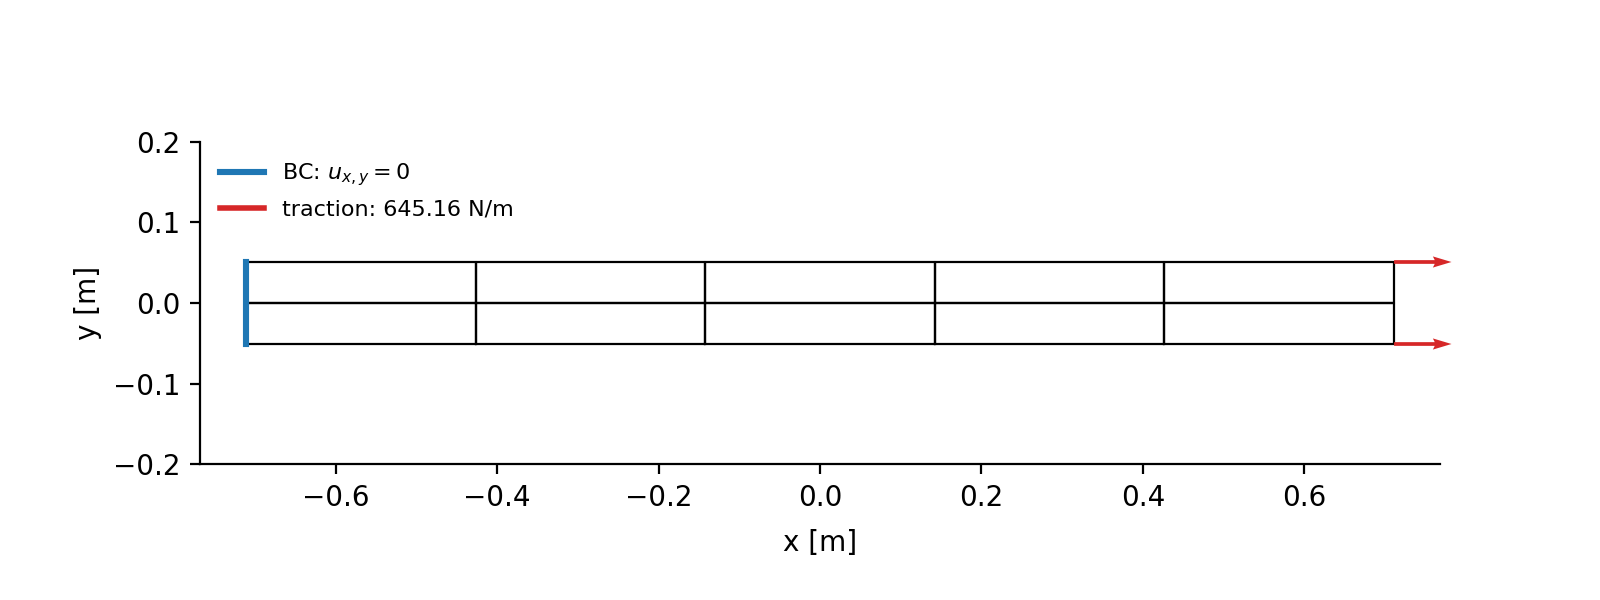
\includegraphics[width=\linewidth]{../figures/panel/case1_n10_undeformed.png}
\caption{$n=10$ undeformed}
\end{subfigure}
\begin{subfigure}{0.32\textwidth}\centering
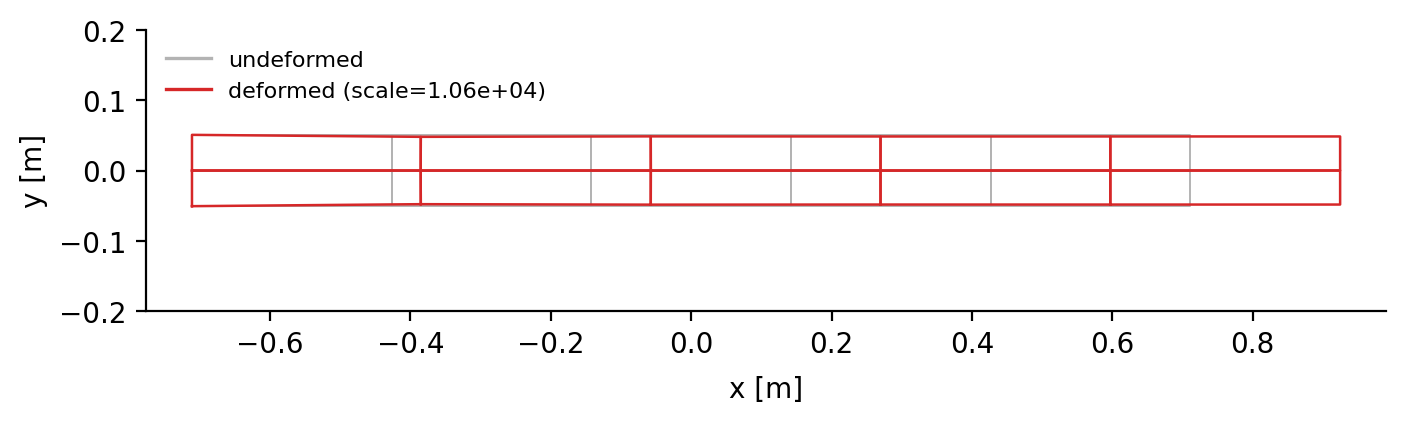
\includegraphics[width=\linewidth]{../figures/panel/case1_n10_deformed.png}
\caption{$n=10$ deformed}
\end{subfigure}
\begin{subfigure}{0.32\textwidth}\centering
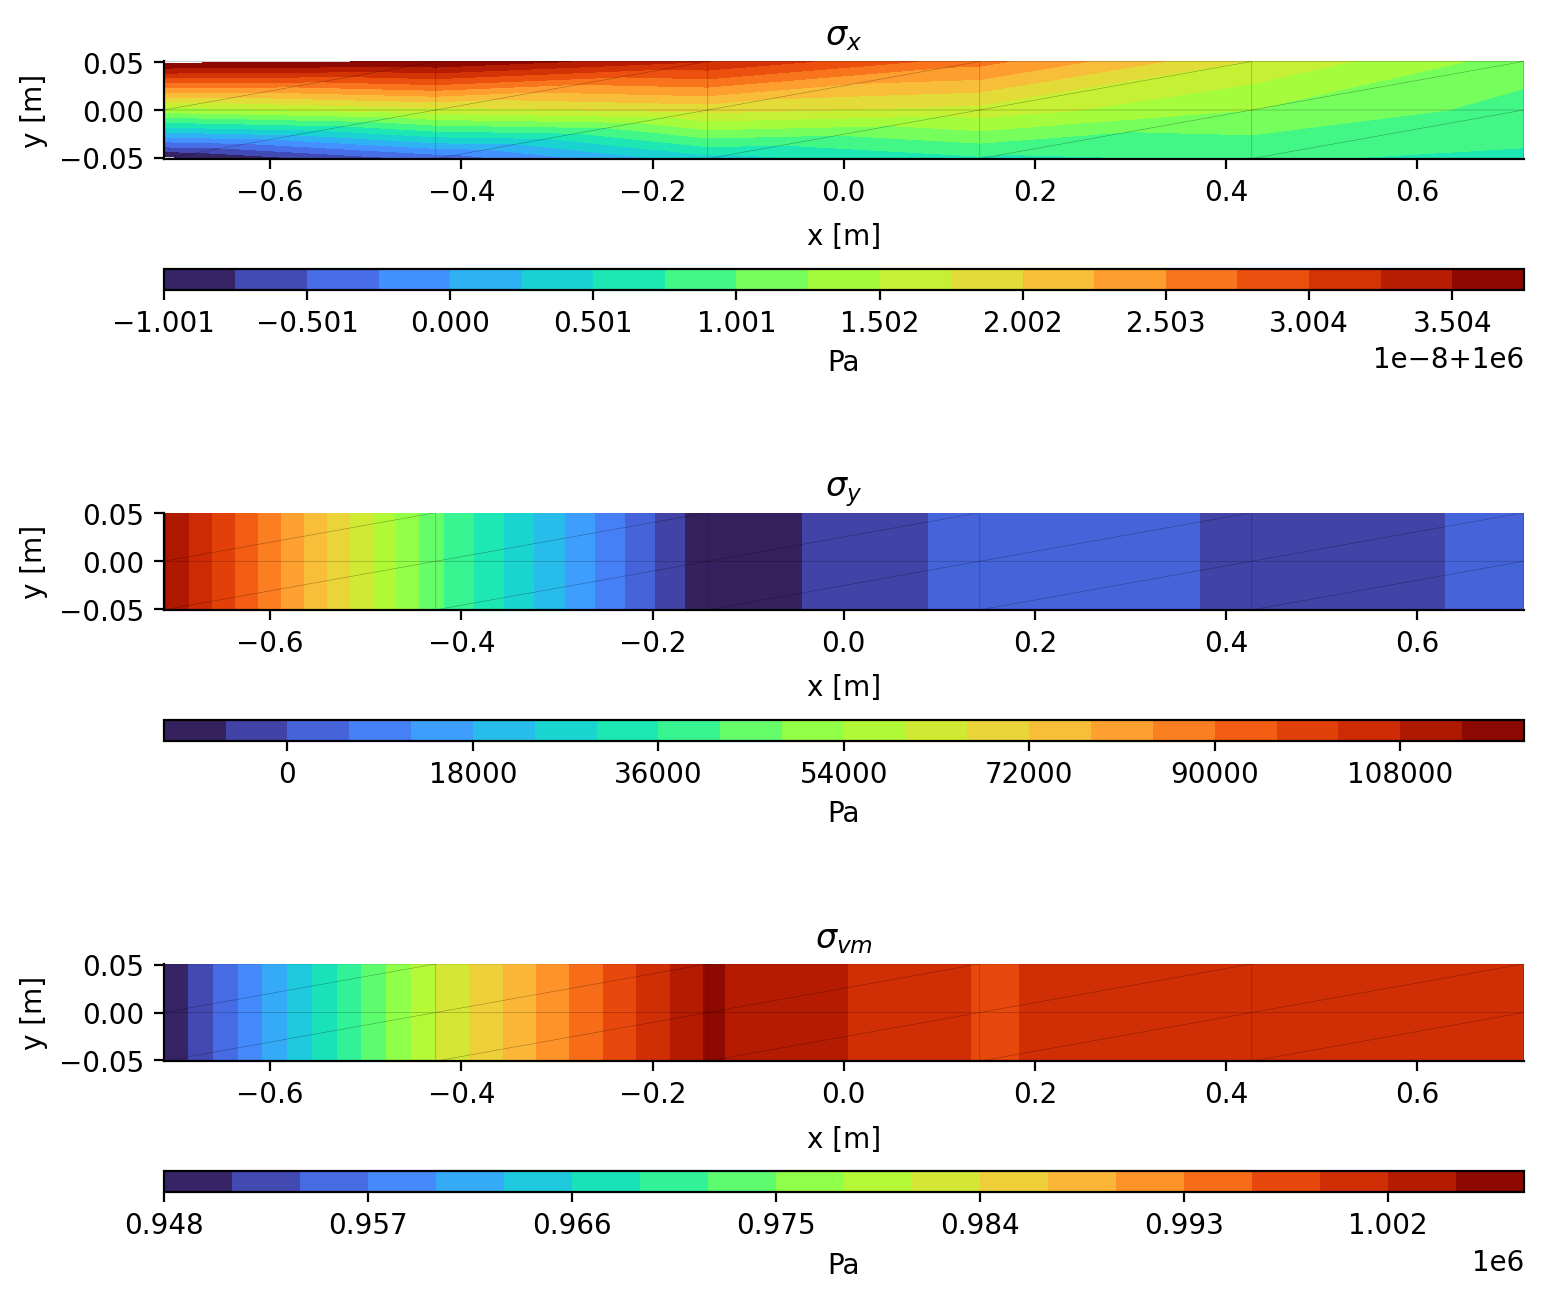
\includegraphics[width=\linewidth]{../figures/panel/case1_n10_stress_stack.png}
\caption{$n=10$ stress stack}
\end{subfigure}
\caption{Case 1 panel results, $n=10$.}
\end{figure}

\begin{figure}[htbp]
\centering
\begin{subfigure}{0.32\textwidth}\centering
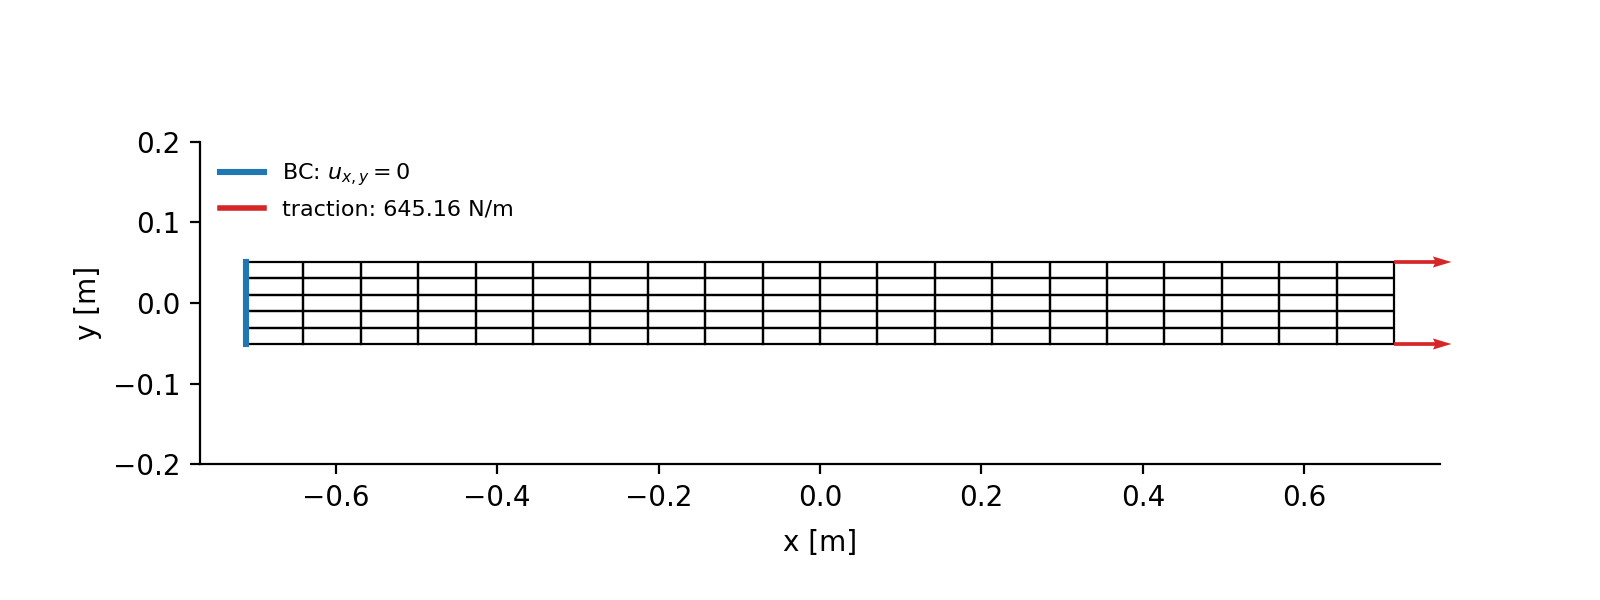
\includegraphics[width=\linewidth]{../figures/panel/case1_n100_undeformed.png}
\caption{$n=100$ undeformed}
\end{subfigure}
\begin{subfigure}{0.32\textwidth}\centering
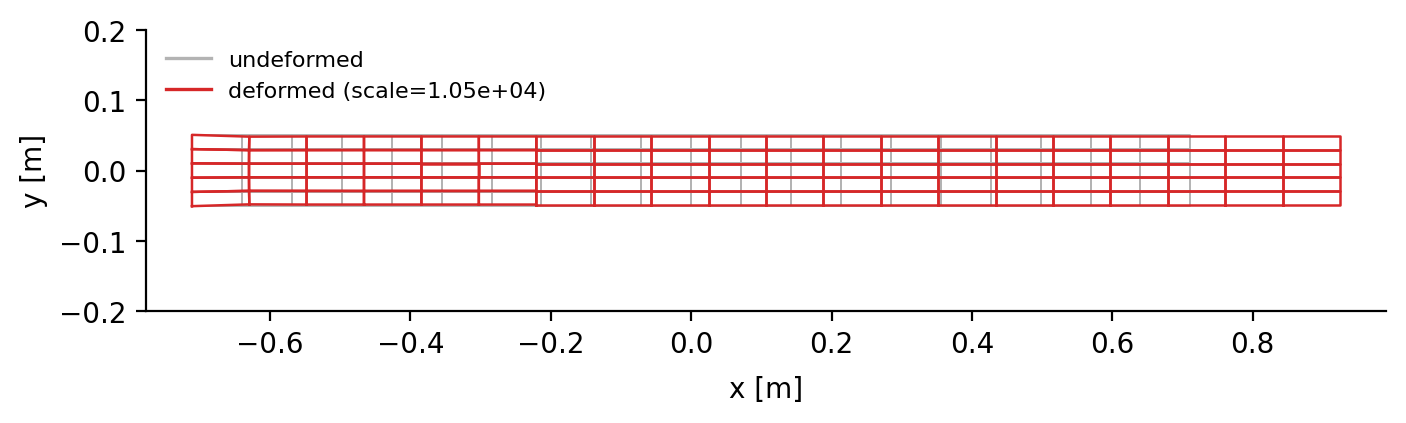
\includegraphics[width=\linewidth]{../figures/panel/case1_n100_deformed.png}
\caption{$n=100$ deformed}
\end{subfigure}
\begin{subfigure}{0.32\textwidth}\centering
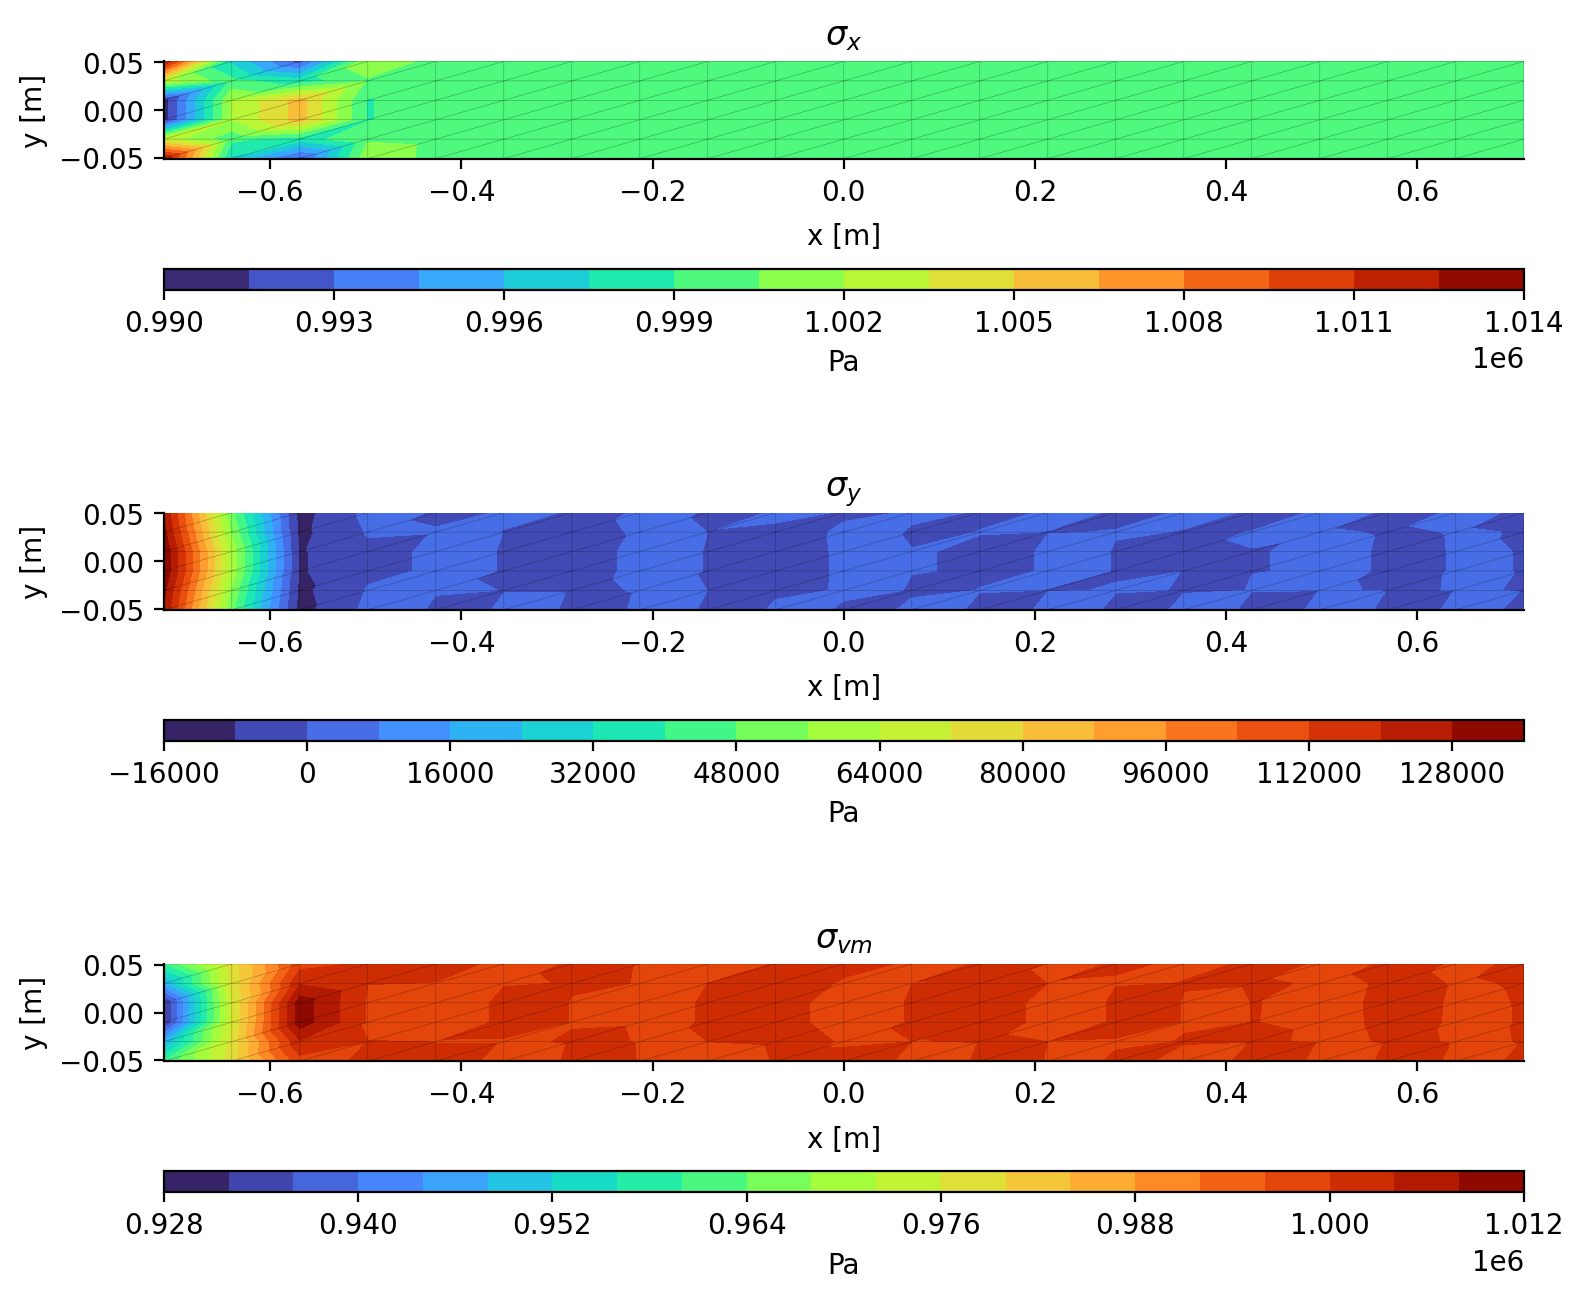
\includegraphics[width=\linewidth]{../figures/panel/case1_n100_stress_stack.png}
\caption{$n=100$ stress stack}
\end{subfigure}
\caption{Case 1 panel results, $n=100$.}
\end{figure}

\begin{figure}[htbp]
\centering
\begin{subfigure}{0.32\textwidth}\centering
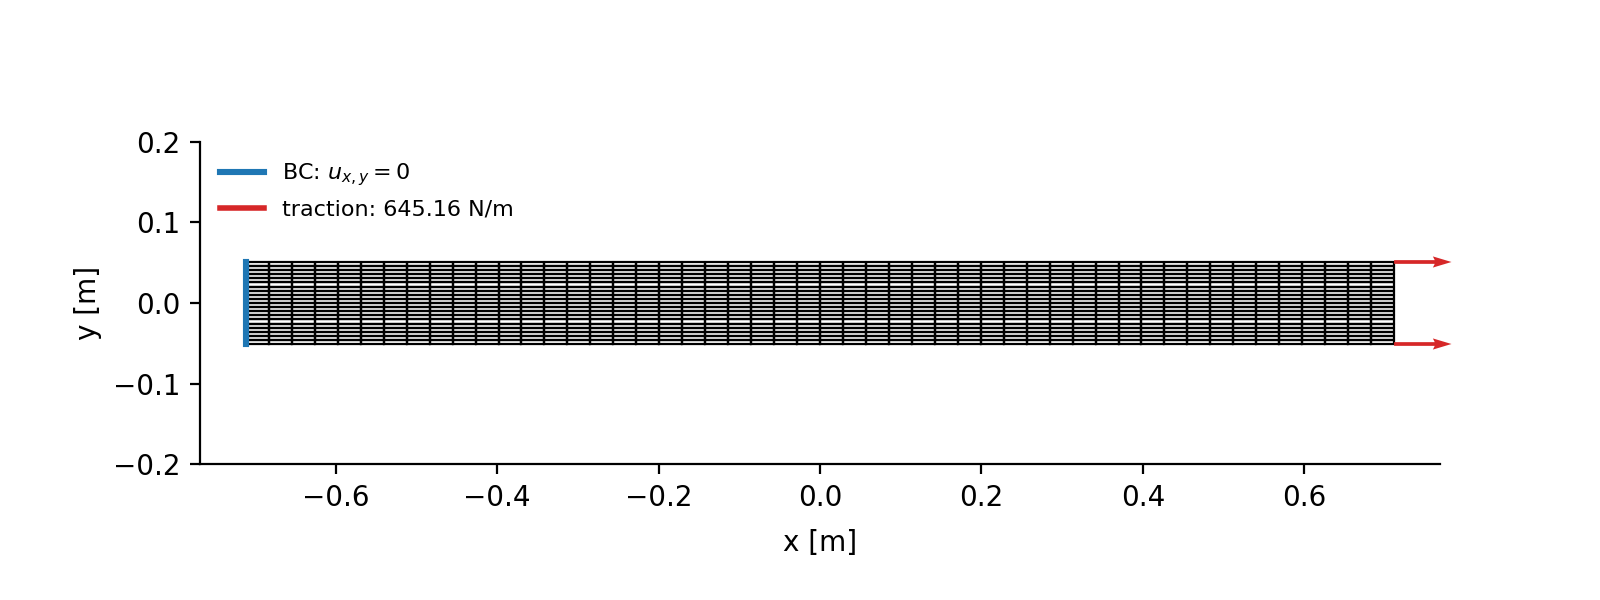
\includegraphics[width=\linewidth]{../figures/panel/case1_n1000_undeformed.png}
\caption{$n=1000$ undeformed}
\end{subfigure}
\begin{subfigure}{0.32\textwidth}\centering
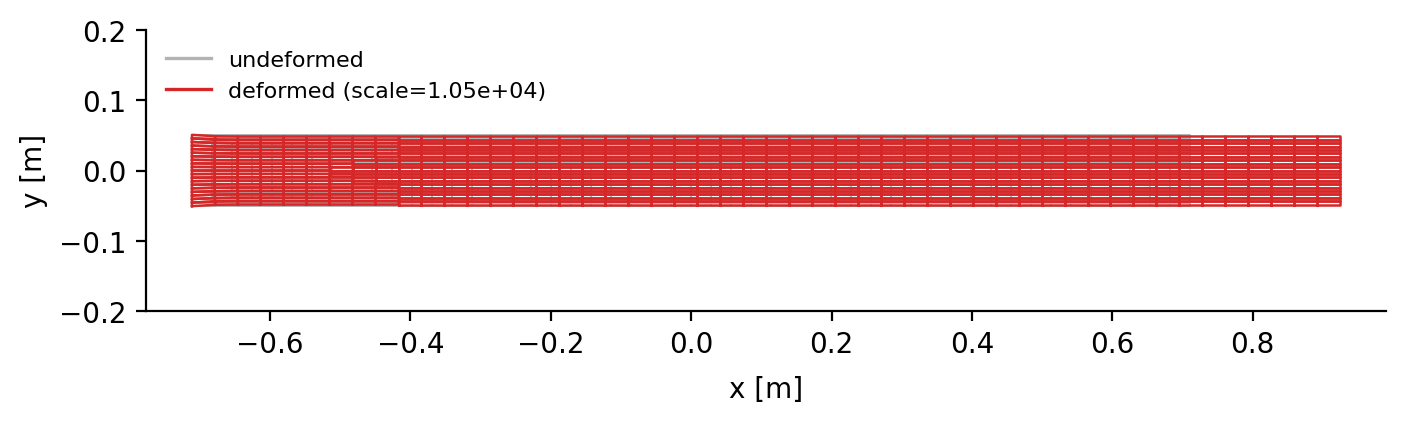
\includegraphics[width=\linewidth]{../figures/panel/case1_n1000_deformed.png}
\caption{$n=1000$ deformed}
\end{subfigure}
\begin{subfigure}{0.32\textwidth}\centering
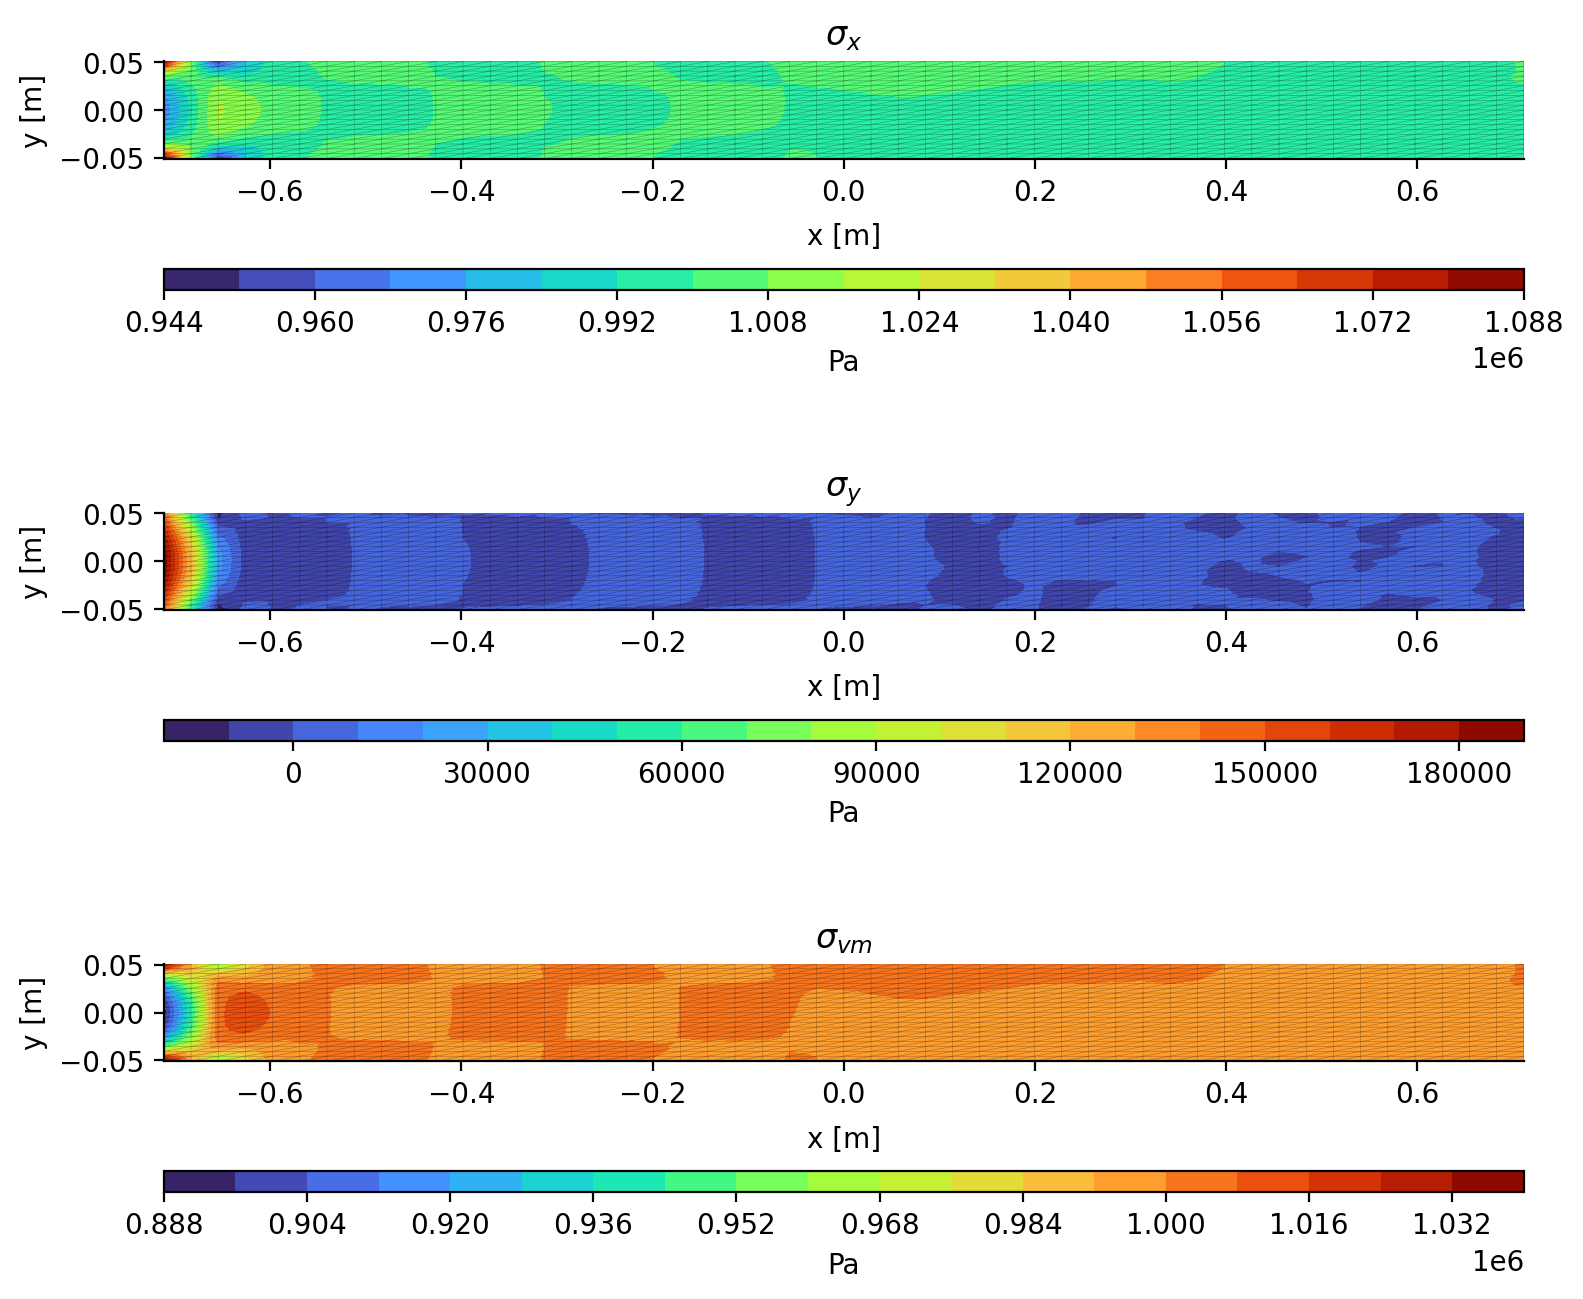
\includegraphics[width=\linewidth]{../figures/panel/case1_n1000_stress_stack.png}
\caption{$n=1000$ stress stack}
\end{subfigure}
\caption{Case 1 panel results, $n=1000$.}
\end{figure}

\clearpage
\subsubsection*{Case 2}
\begin{figure}[htbp]
\centering
\begin{subfigure}{0.32\textwidth}\centering
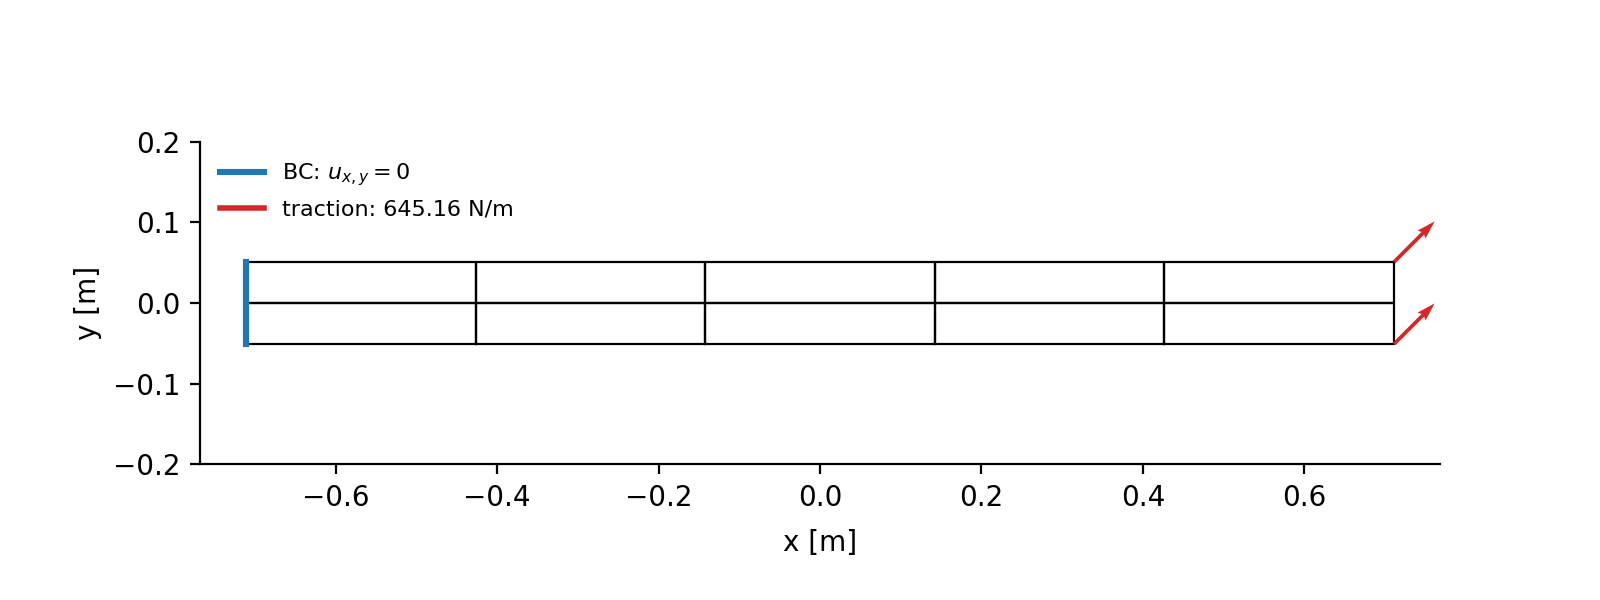
\includegraphics[width=\linewidth]{../figures/panel/case2_n10_undeformed.png}
\caption{$n=10$ undeformed}
\end{subfigure}
\begin{subfigure}{0.32\textwidth}\centering
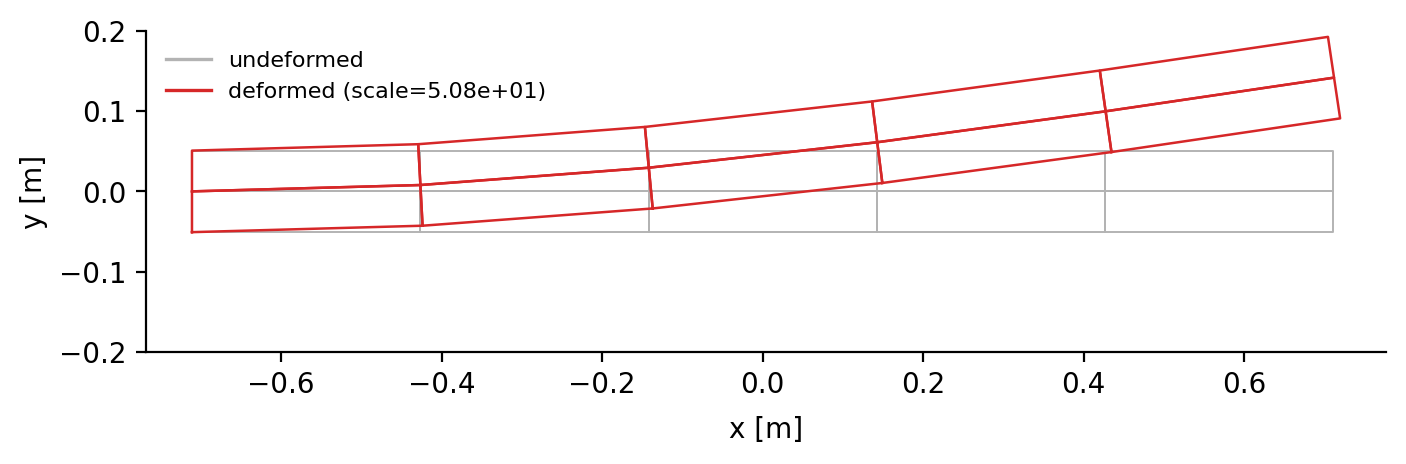
\includegraphics[width=\linewidth]{../figures/panel/case2_n10_deformed.png}
\caption{$n=10$ deformed}
\end{subfigure}
\begin{subfigure}{0.32\textwidth}\centering
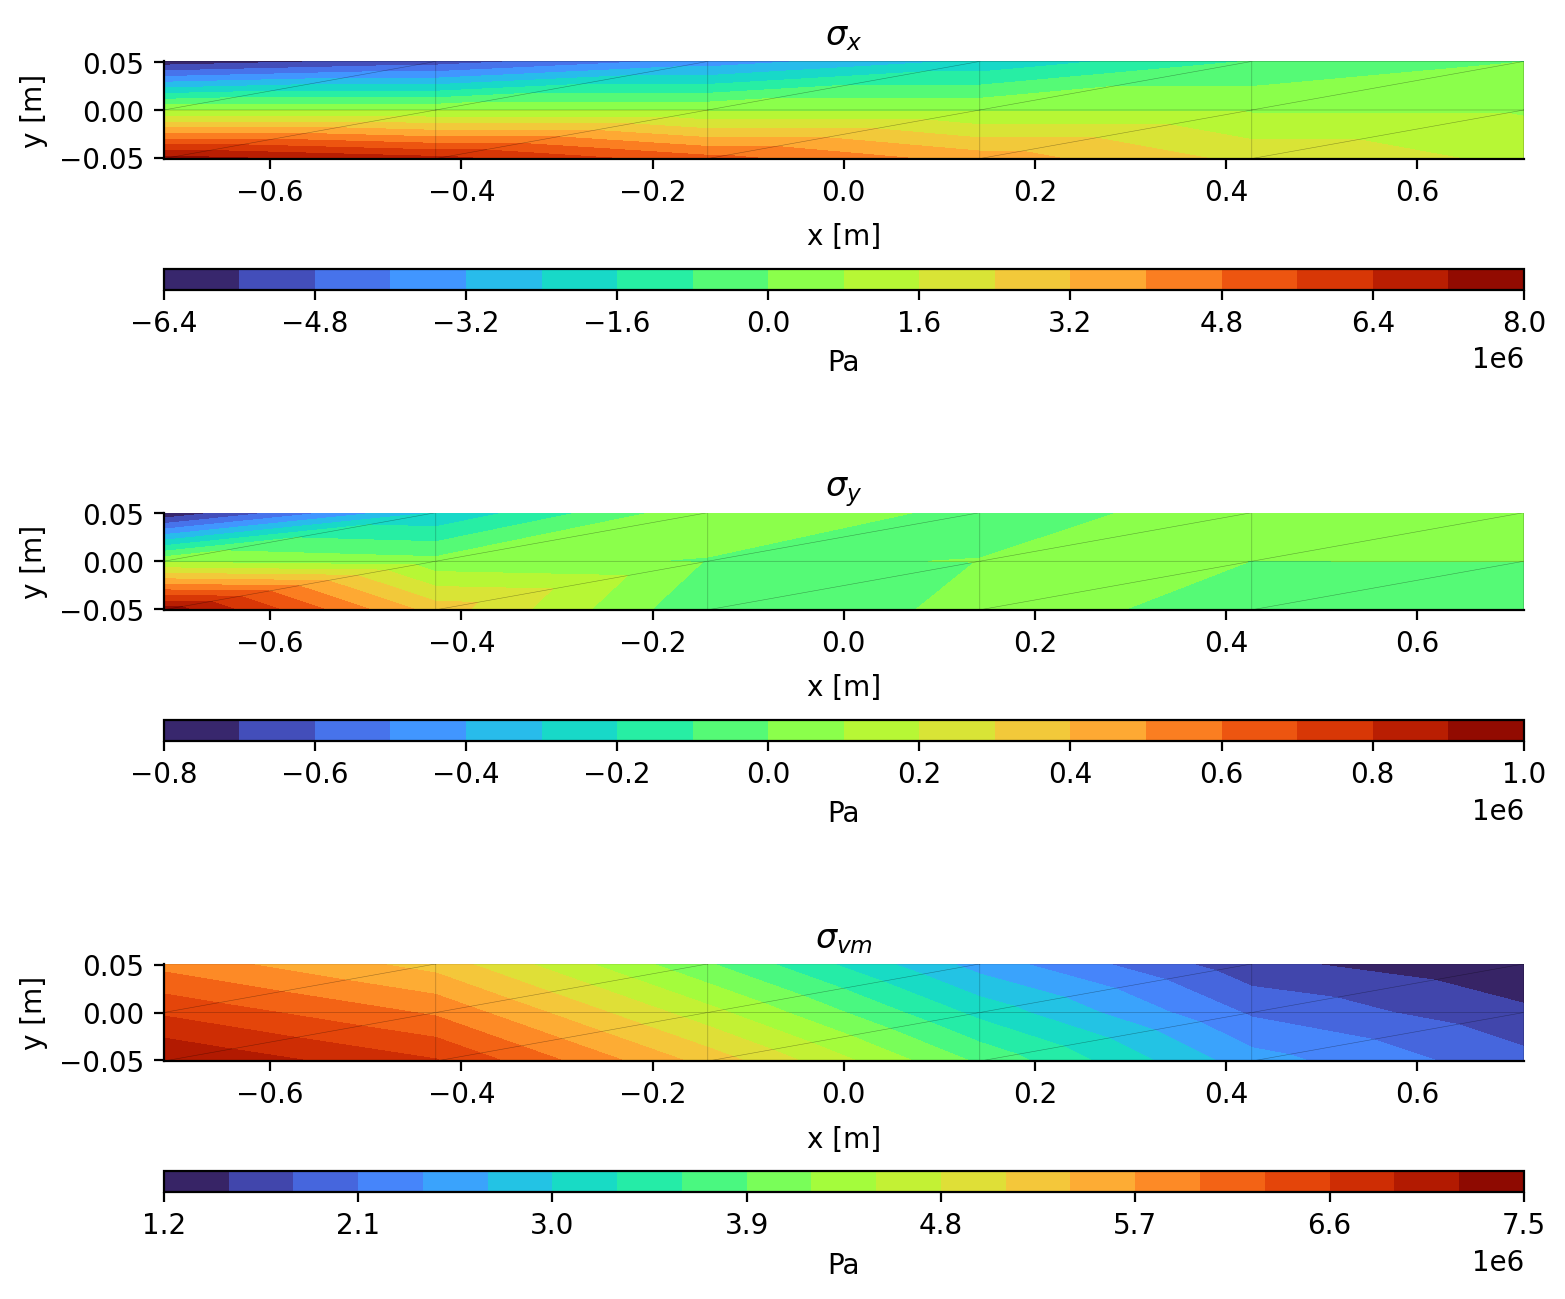
\includegraphics[width=\linewidth]{../figures/panel/case2_n10_stress_stack.png}
\caption{$n=10$ stress stack}
\end{subfigure}
\caption{Case 2 panel results, $n=10$.}
\end{figure}

\begin{figure}[htbp]
\centering
\begin{subfigure}{0.32\textwidth}\centering
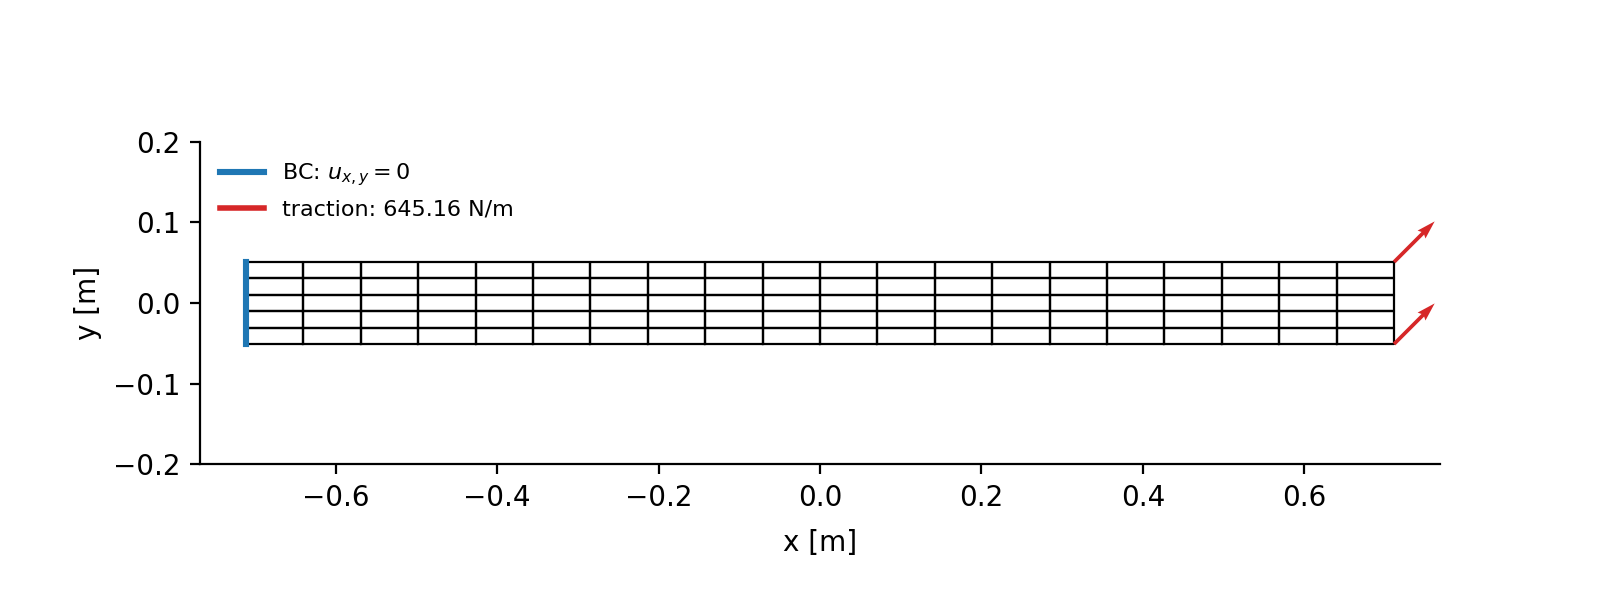
\includegraphics[width=\linewidth]{../figures/panel/case2_n100_undeformed.png}
\caption{$n=100$ undeformed}
\end{subfigure}
\begin{subfigure}{0.32\textwidth}\centering
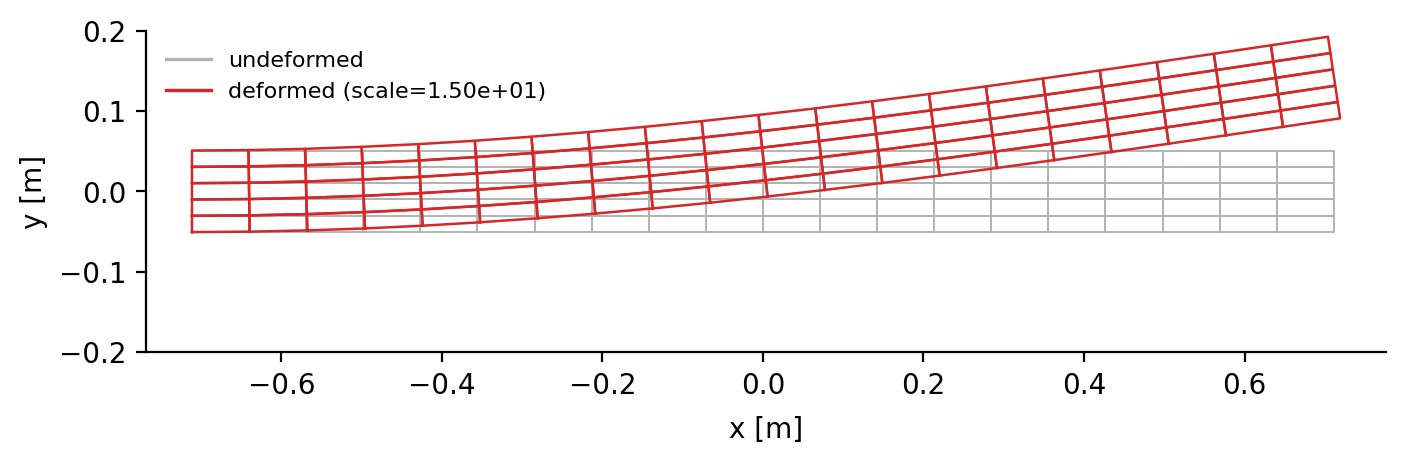
\includegraphics[width=\linewidth]{../figures/panel/case2_n100_deformed.png}
\caption{$n=100$ deformed}
\end{subfigure}
\begin{subfigure}{0.32\textwidth}\centering
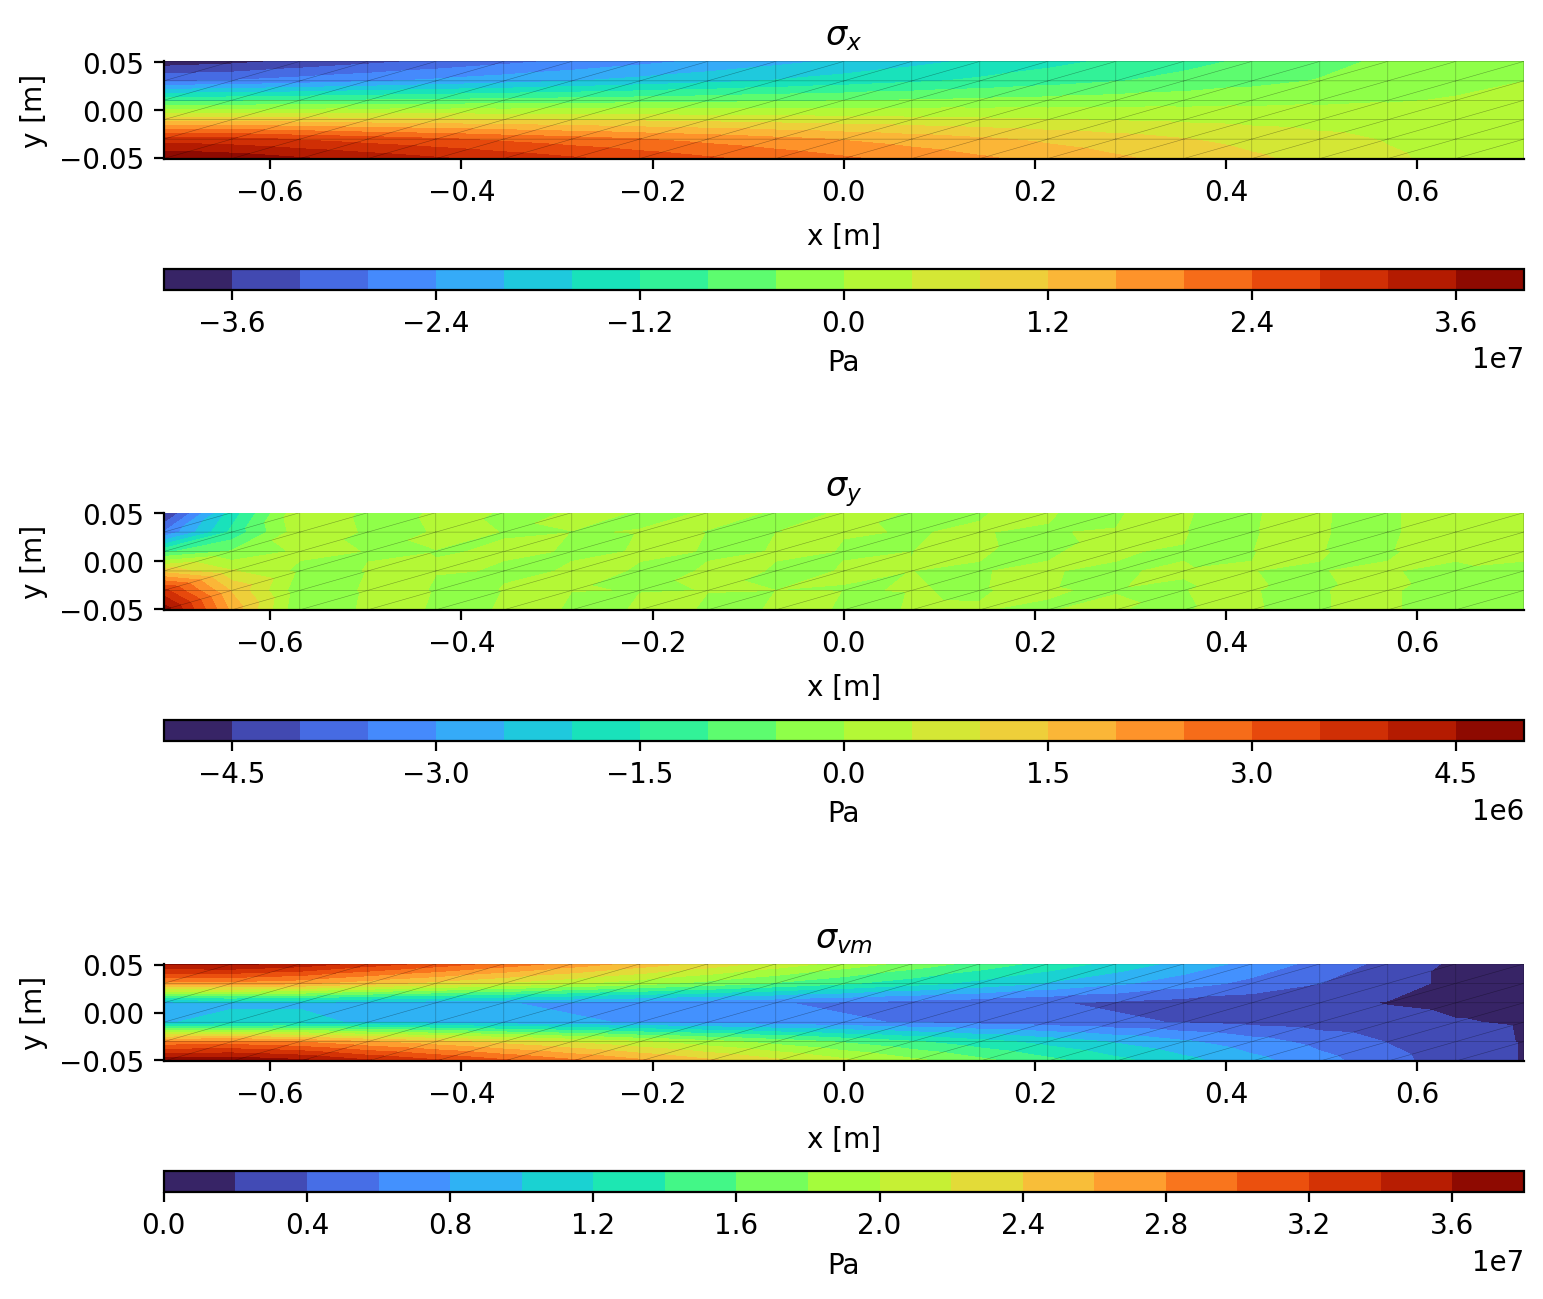
\includegraphics[width=\linewidth]{../figures/panel/case2_n100_stress_stack.png}
\caption{$n=100$ stress stack}
\end{subfigure}
\caption{Case 2 panel results, $n=100$.}
\end{figure}

\begin{figure}[htbp]
\centering
\begin{subfigure}{0.32\textwidth}\centering
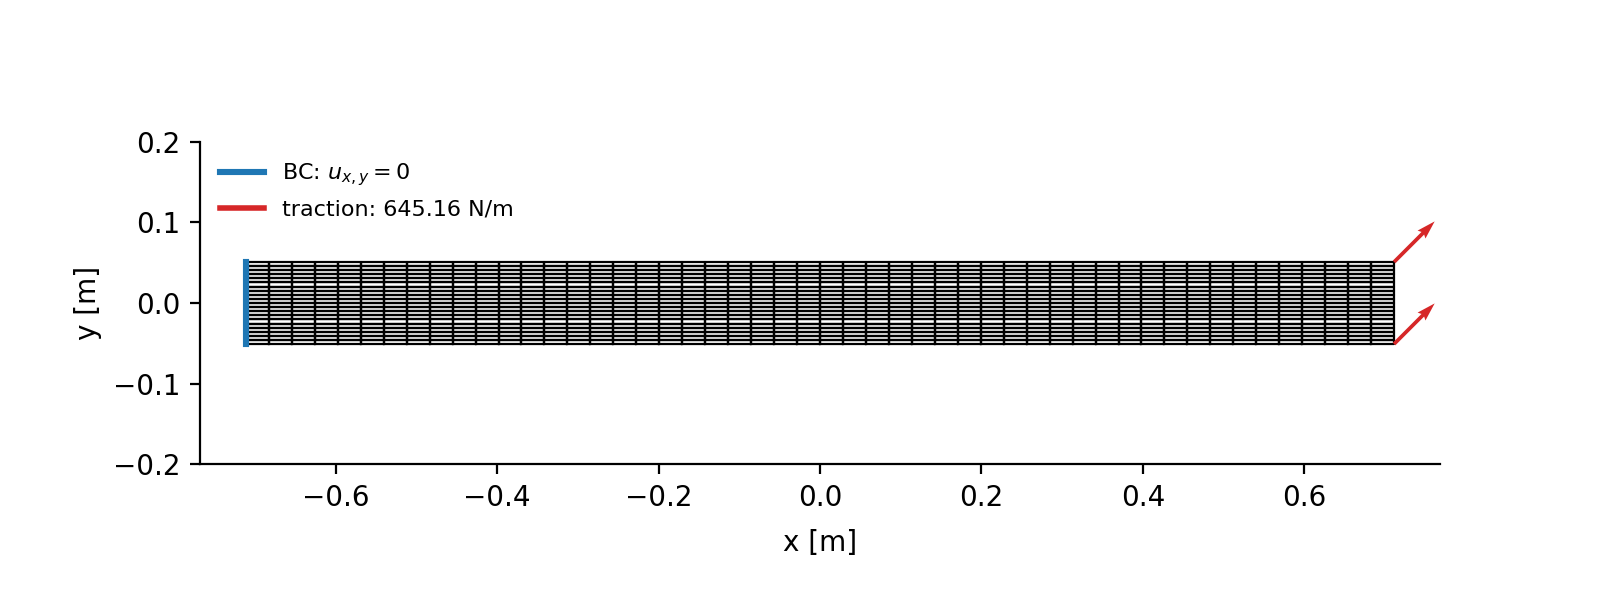
\includegraphics[width=\linewidth]{../figures/panel/case2_n1000_undeformed.png}
\caption{$n=1000$ undeformed}
\end{subfigure}
\begin{subfigure}{0.32\textwidth}\centering
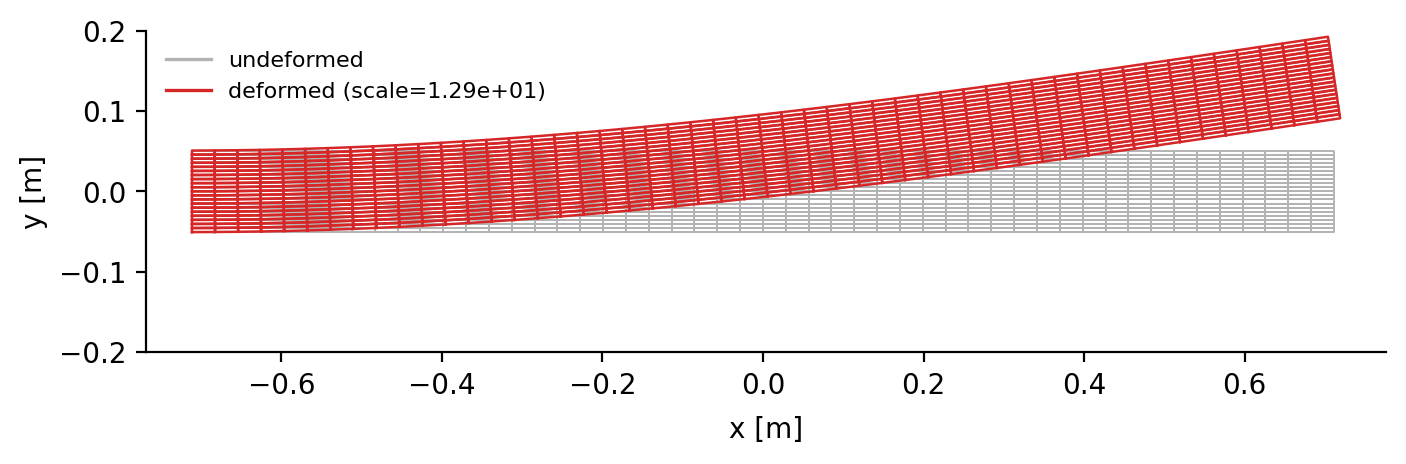
\includegraphics[width=\linewidth]{../figures/panel/case2_n1000_deformed.png}
\caption{$n=1000$ deformed}
\end{subfigure}
\begin{subfigure}{0.32\textwidth}\centering
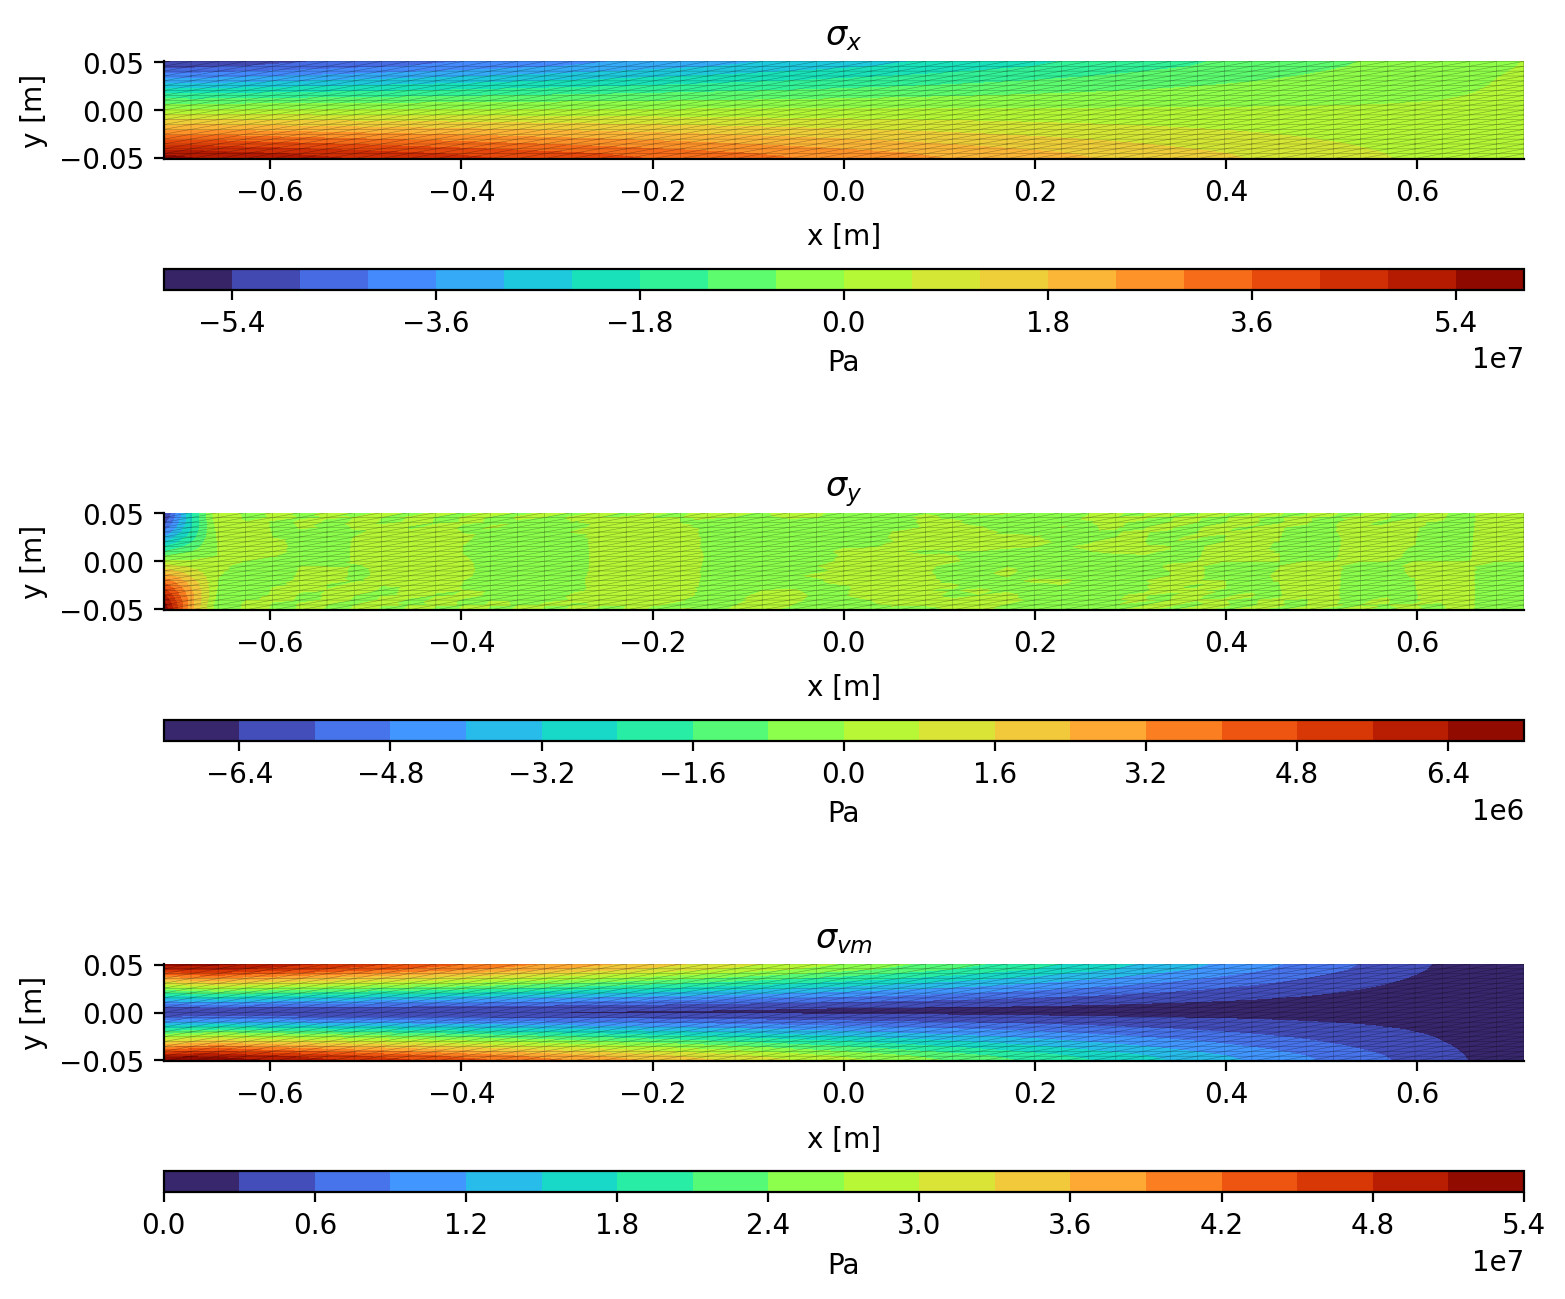
\includegraphics[width=\linewidth]{../figures/panel/case2_n1000_stress_stack.png}
\caption{$n=1000$ stress stack}
\end{subfigure}
\caption{Case 2 panel results, $n=1000$.}
\end{figure}

\clearpage
\subsubsection*{Case 3}
\begin{figure}[htbp]
\centering
\begin{subfigure}{0.32\textwidth}\centering
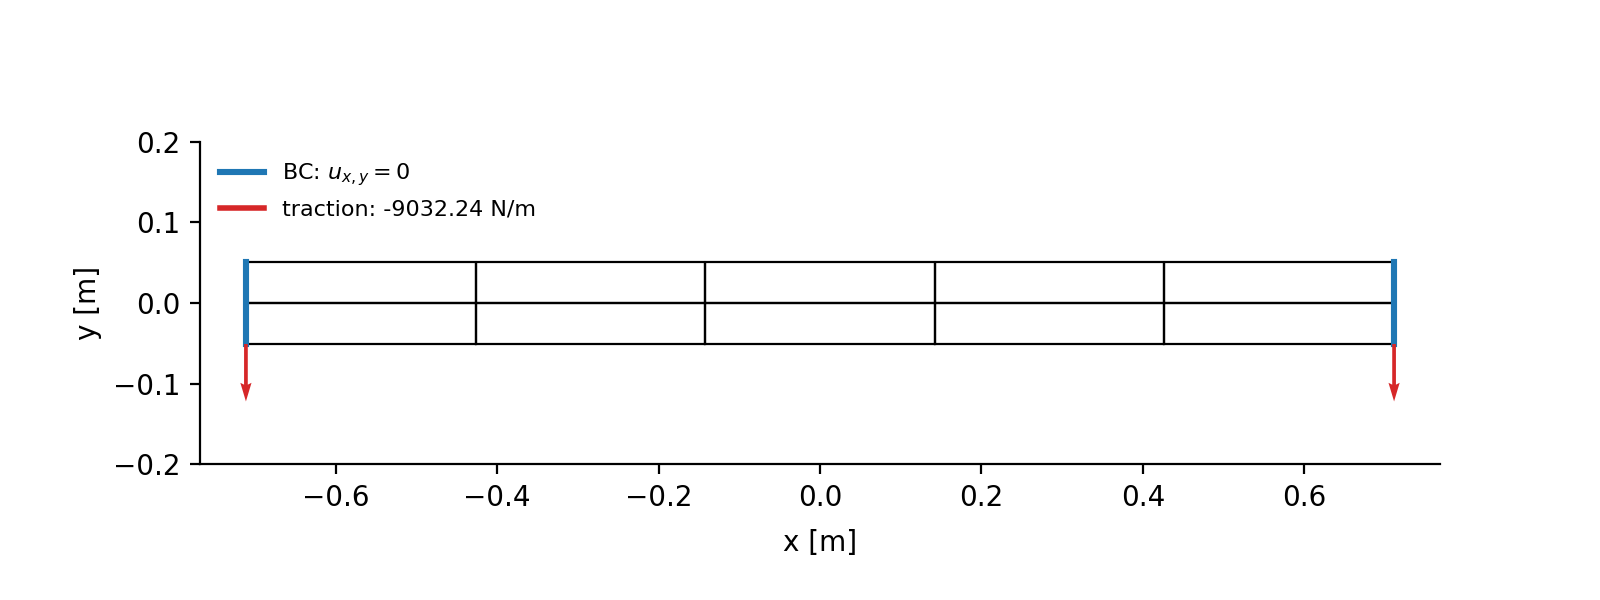
\includegraphics[width=\linewidth]{../figures/panel/case3_n10_undeformed.png}
\caption{$n=10$ undeformed}
\end{subfigure}
\begin{subfigure}{0.32\textwidth}\centering
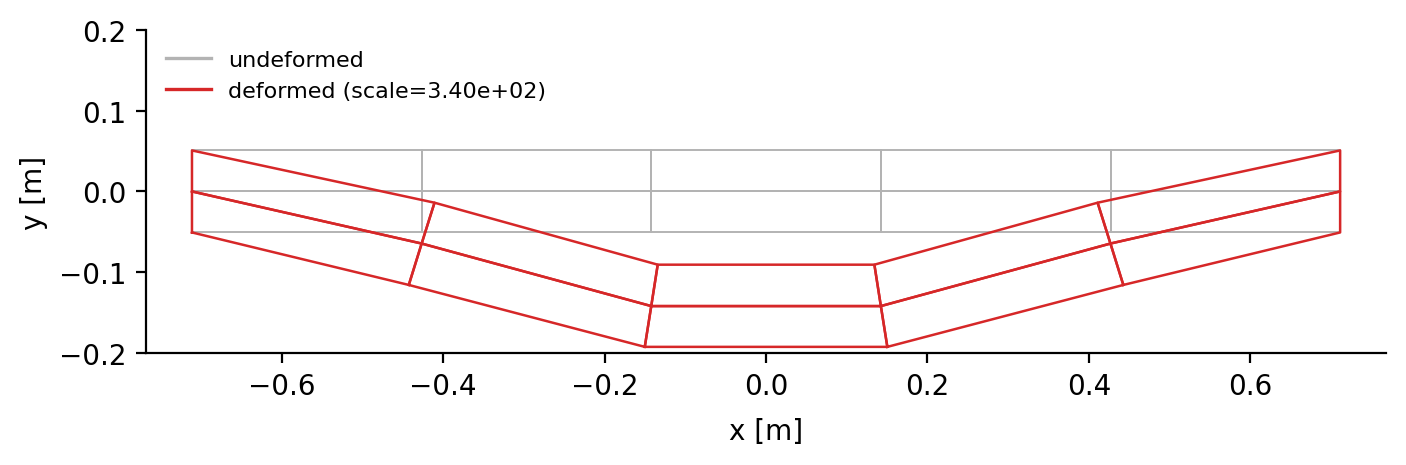
\includegraphics[width=\linewidth]{../figures/panel/case3_n10_deformed.png}
\caption{$n=10$ deformed}
\end{subfigure}
\begin{subfigure}{0.32\textwidth}\centering
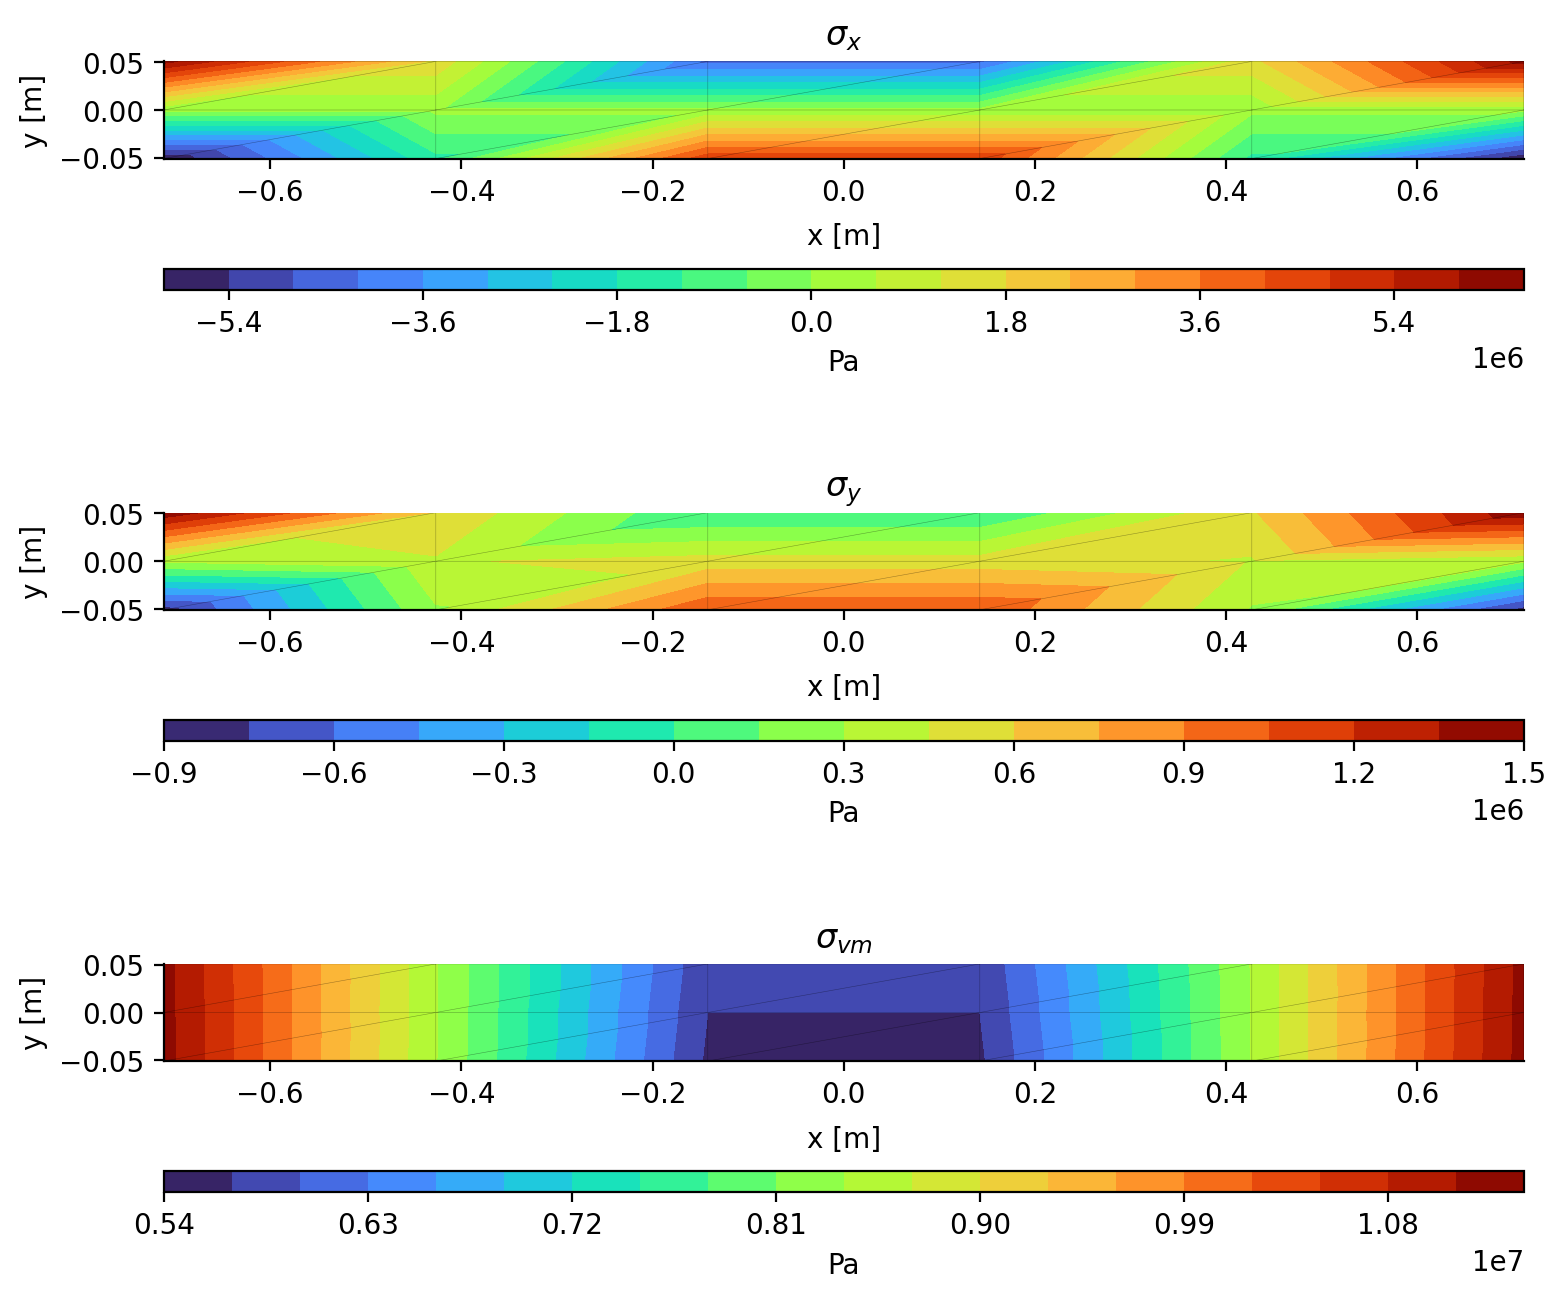
\includegraphics[width=\linewidth]{../figures/panel/case3_n10_stress_stack.png}
\caption{$n=10$ stress stack}
\end{subfigure}
\caption{Case 3 panel results, $n=10$.}
\end{figure}

\begin{figure}[htbp]
\centering
\begin{subfigure}{0.32\textwidth}\centering
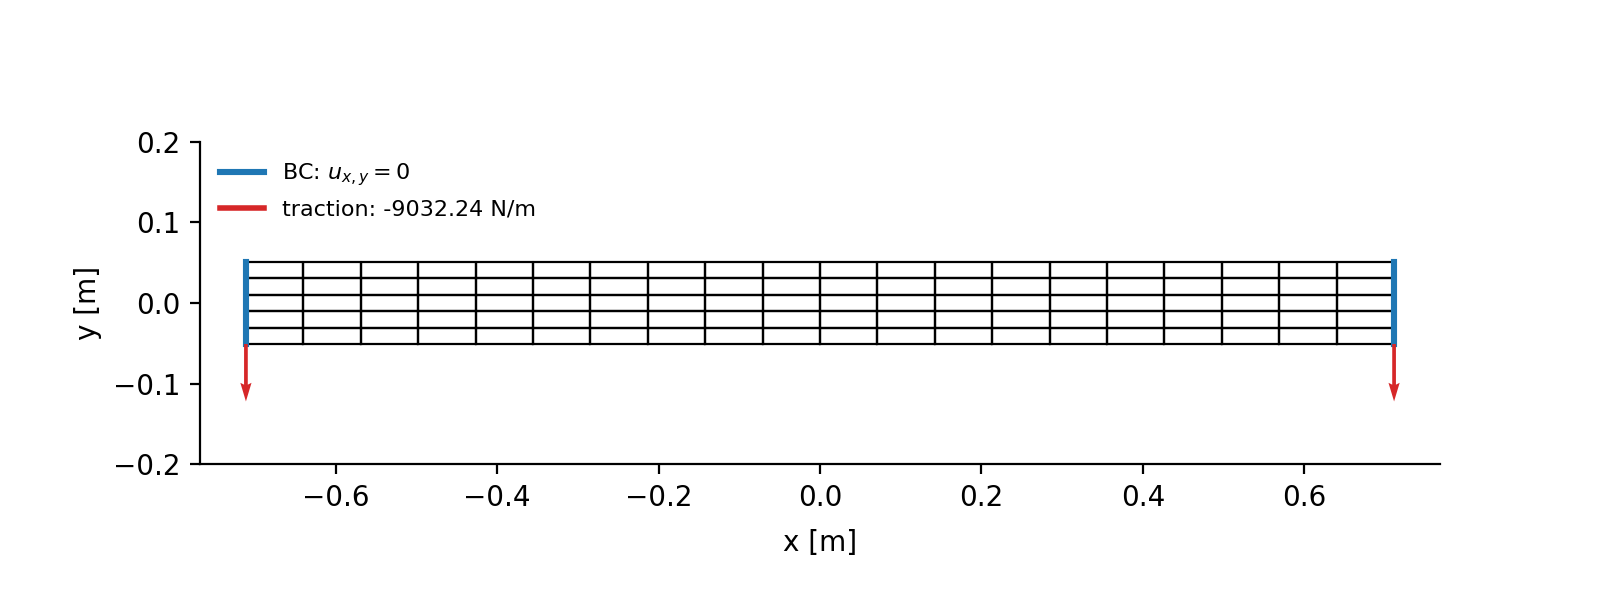
\includegraphics[width=\linewidth]{../figures/panel/case3_n100_undeformed.png}
\caption{$n=100$ undeformed}
\end{subfigure}
\begin{subfigure}{0.32\textwidth}\centering
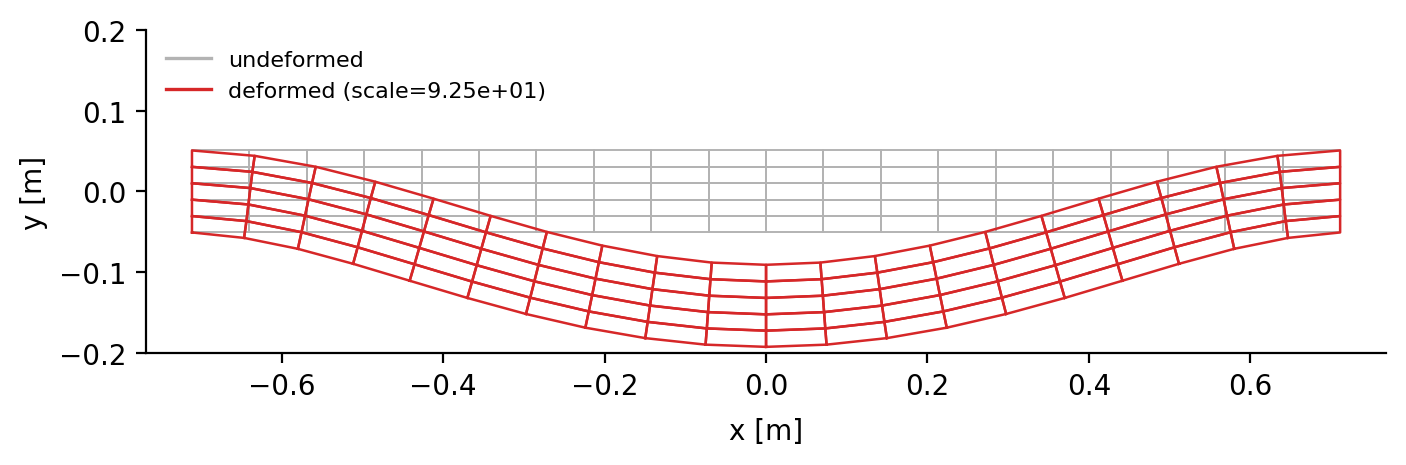
\includegraphics[width=\linewidth]{../figures/panel/case3_n100_deformed.png}
\caption{$n=100$ deformed}
\end{subfigure}
\begin{subfigure}{0.32\textwidth}\centering
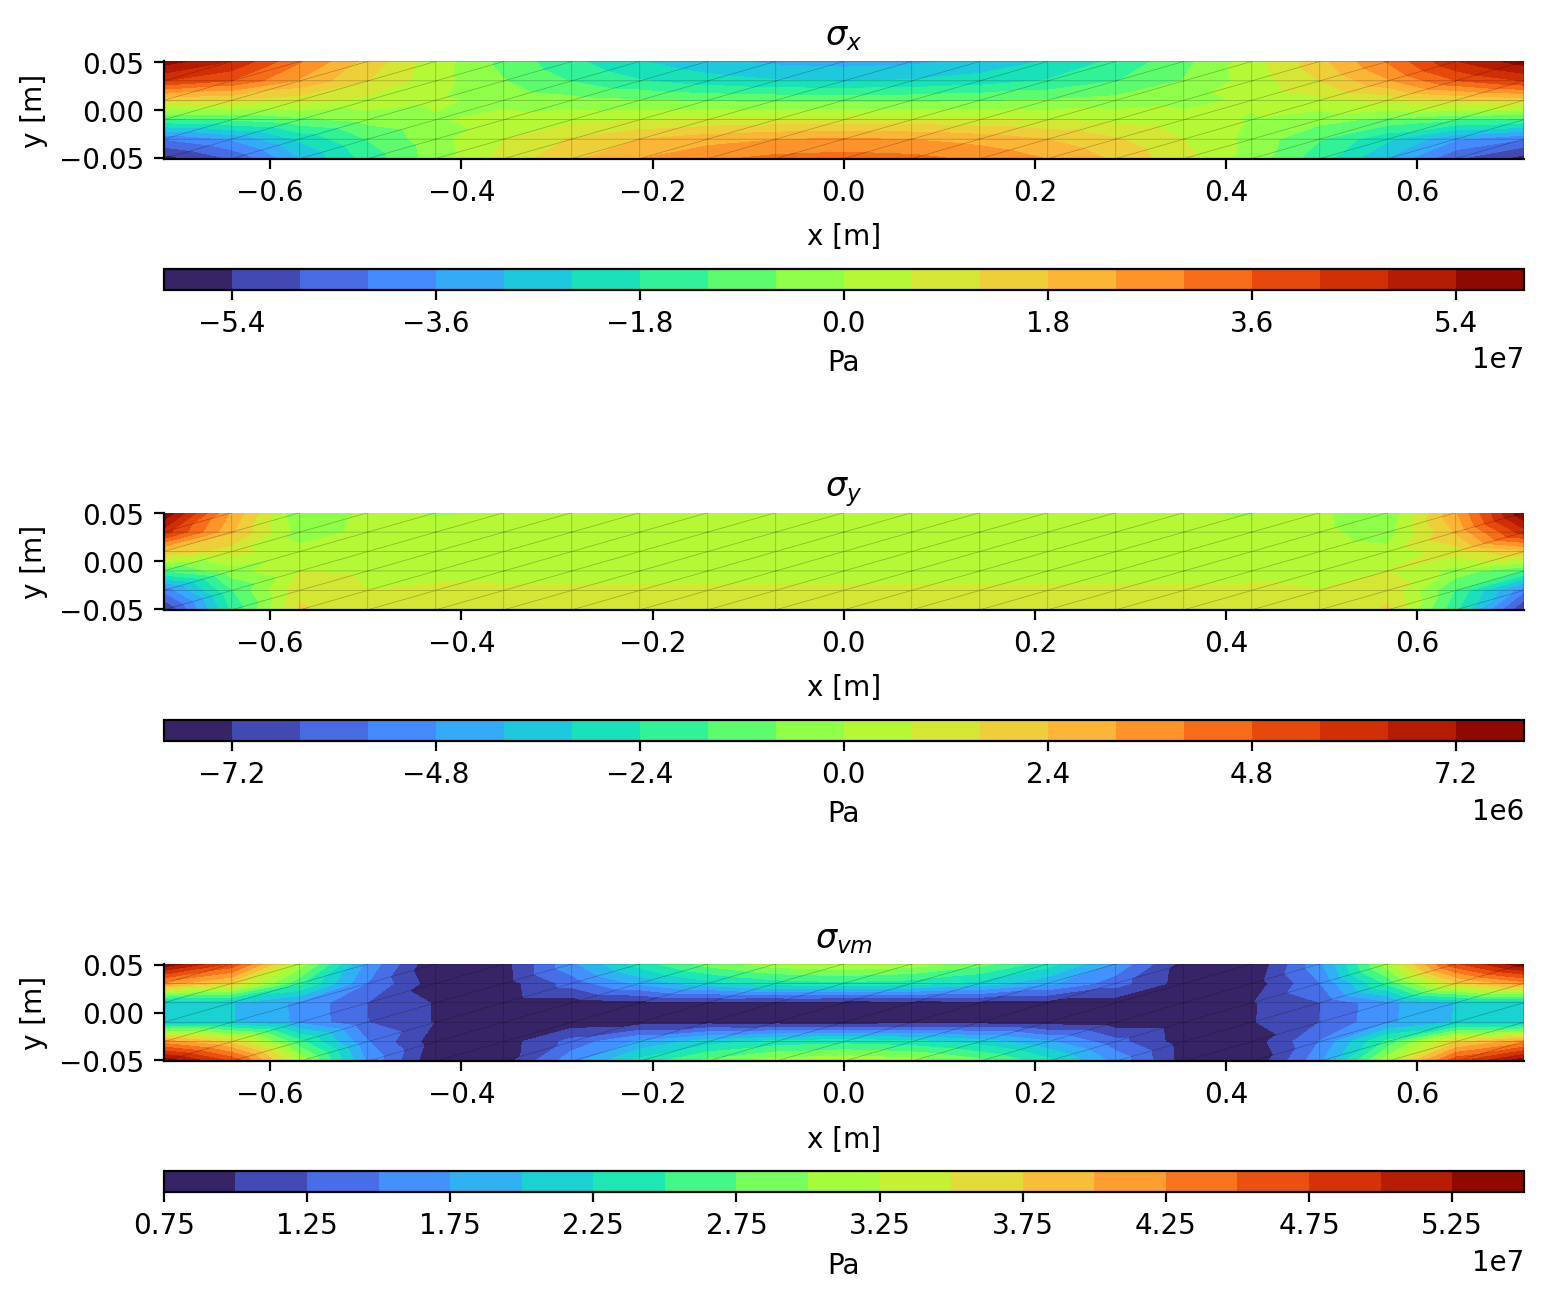
\includegraphics[width=\linewidth]{../figures/panel/case3_n100_stress_stack.png}
\caption{$n=100$ stress stack}
\end{subfigure}
\caption{Case 3 panel results, $n=100$.}
\end{figure}

\begin{figure}[htbp]
\centering
\begin{subfigure}{0.32\textwidth}\centering
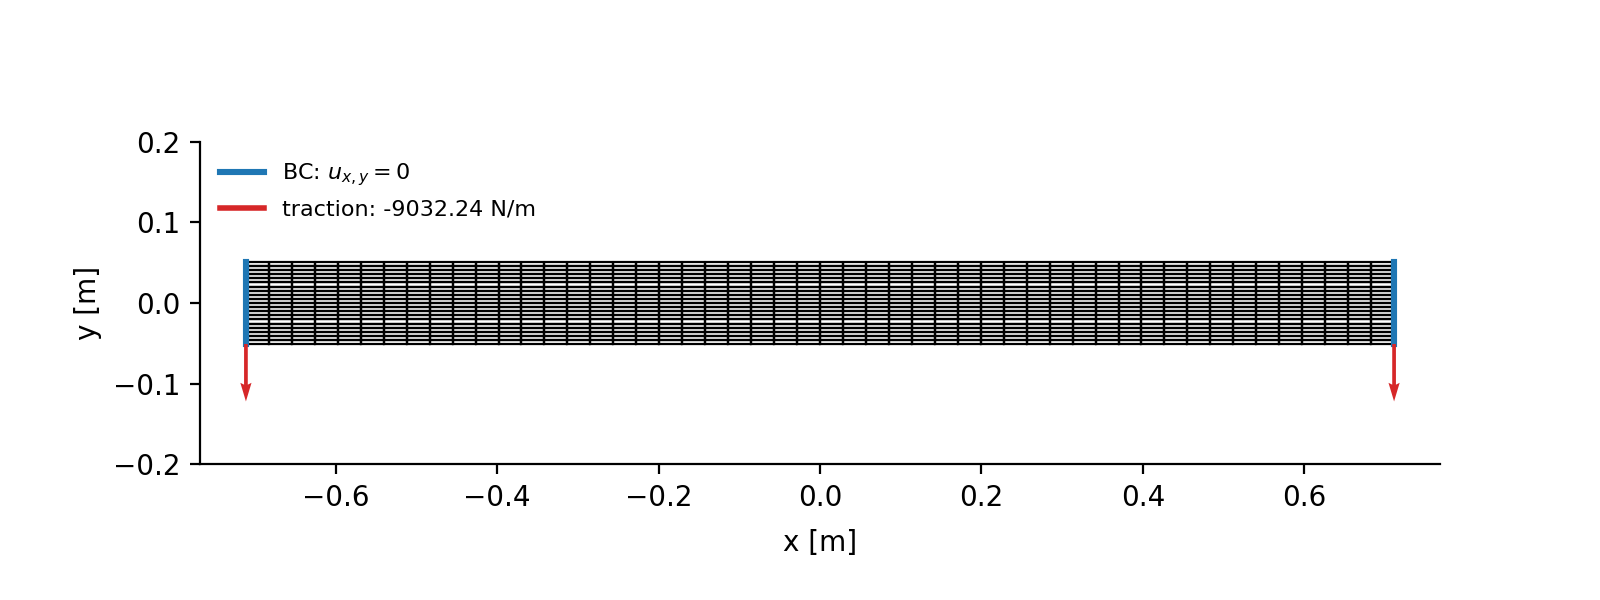
\includegraphics[width=\linewidth]{../figures/panel/case3_n1000_undeformed.png}
\caption{$n=1000$ undeformed}
\end{subfigure}
\begin{subfigure}{0.32\textwidth}\centering
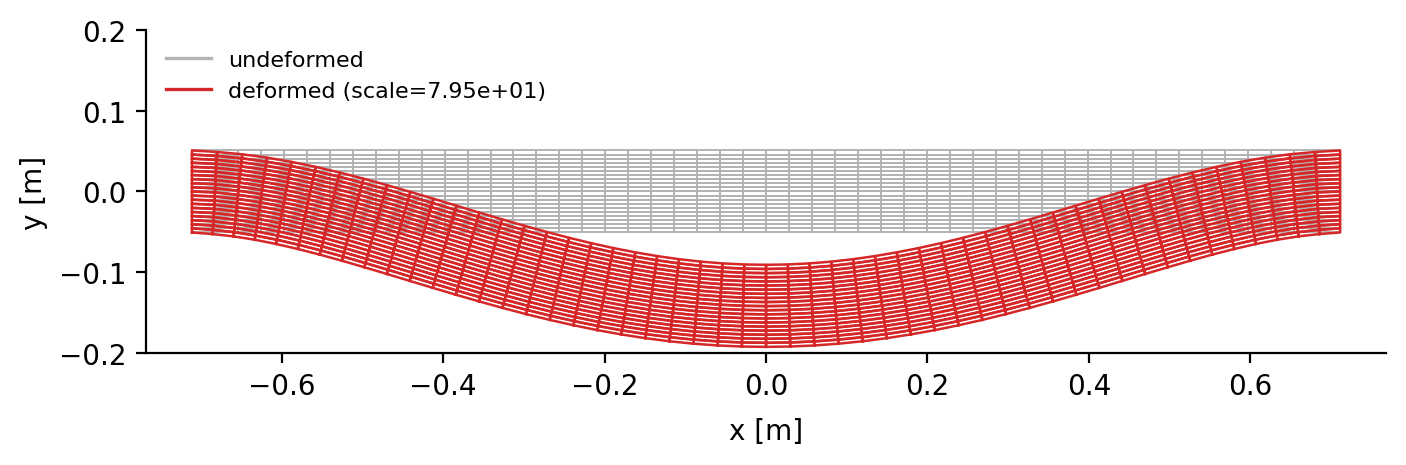
\includegraphics[width=\linewidth]{../figures/panel/case3_n1000_deformed.png}
\caption{$n=1000$ deformed}
\end{subfigure}
\begin{subfigure}{0.32\textwidth}\centering
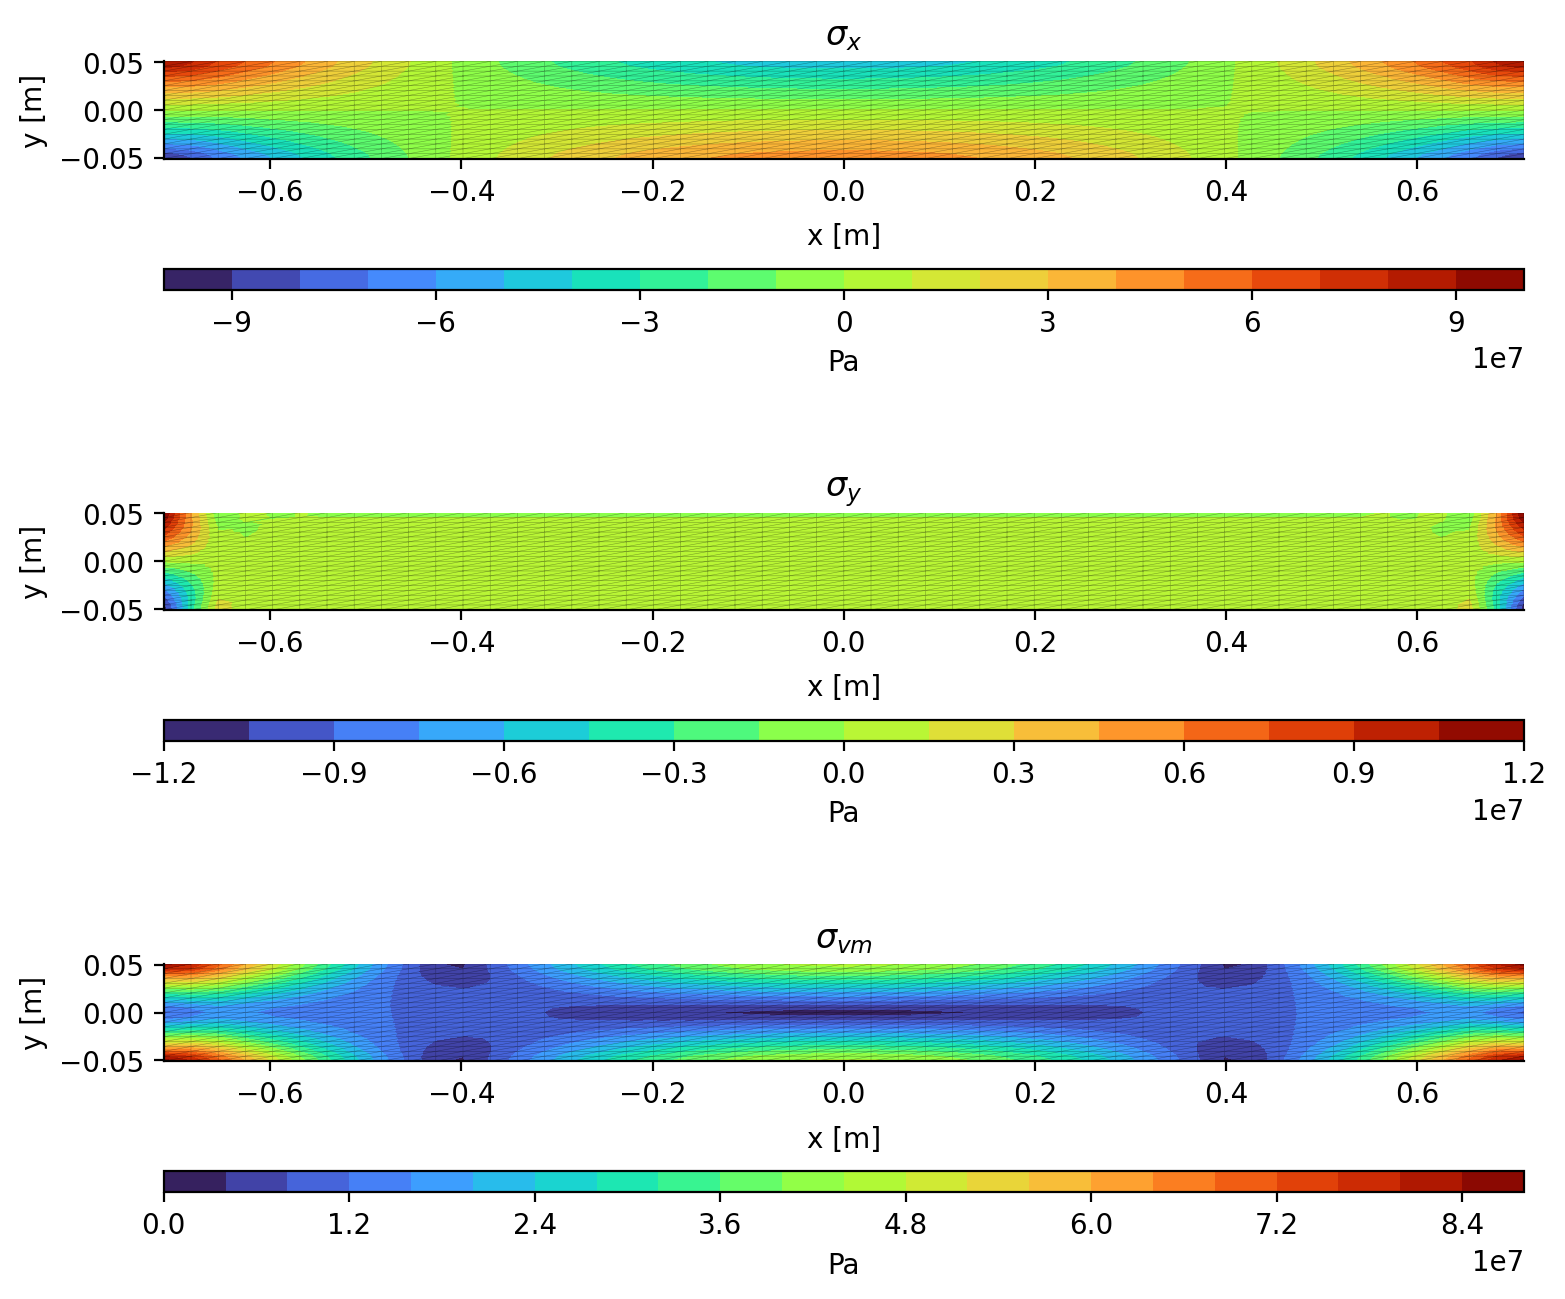
\includegraphics[width=\linewidth]{../figures/panel/case3_n1000_stress_stack.png}
\caption{$n=1000$ stress stack}
\end{subfigure}
\caption{Case 3 panel results, $n=1000$.}
\end{figure}

\clearpage
\section*{Appendix B: Code Listings}
This appendix is intentionally left blank for code listings to be inserted.

\end{document}
